\section{Análise de Centralidade em Grafos de Conectividade}
\label{sec:analise_centralidade}

Nesta seção, investigamos as principais métricas de centralidade (\emph{betweenness}, \emph{degree} e \emph{eigenvector}) em redes de conectividade construídas a partir das métricas CF-PLM (EEG-ECG) e PLI (EEG-EEG). Cada métrica de centralidade oferece uma perspectiva distinta sobre a importância dos nós (canais) na rede \cite{rubinov2010complex, bullmore2009complex}. As redes foram geradas nos cenários \emph{com outliers} e \emph{sem outliers} para verificar a robustez das estruturas. A seguir, descrevemos e interpretamos cada métrica.

\subsection{Betweenness Centrality}
A \emph{betweenness centrality} mede quantas vezes um nó (canal) atua como “ponte” nos caminhos mais curtos entre quaisquer dois nós da rede. Em outras palavras, um canal com alta \emph{betweenness} possui influência considerável sobre o fluxo de informações, pois muitos caminhos de comunicação passam por ele \cite{freeman1977set}.

\subsubsection{CF-PLM (EEG-ECG)}
\begin{figure}[htb]
    \centering
    \subfloat[Com Outliers]{
        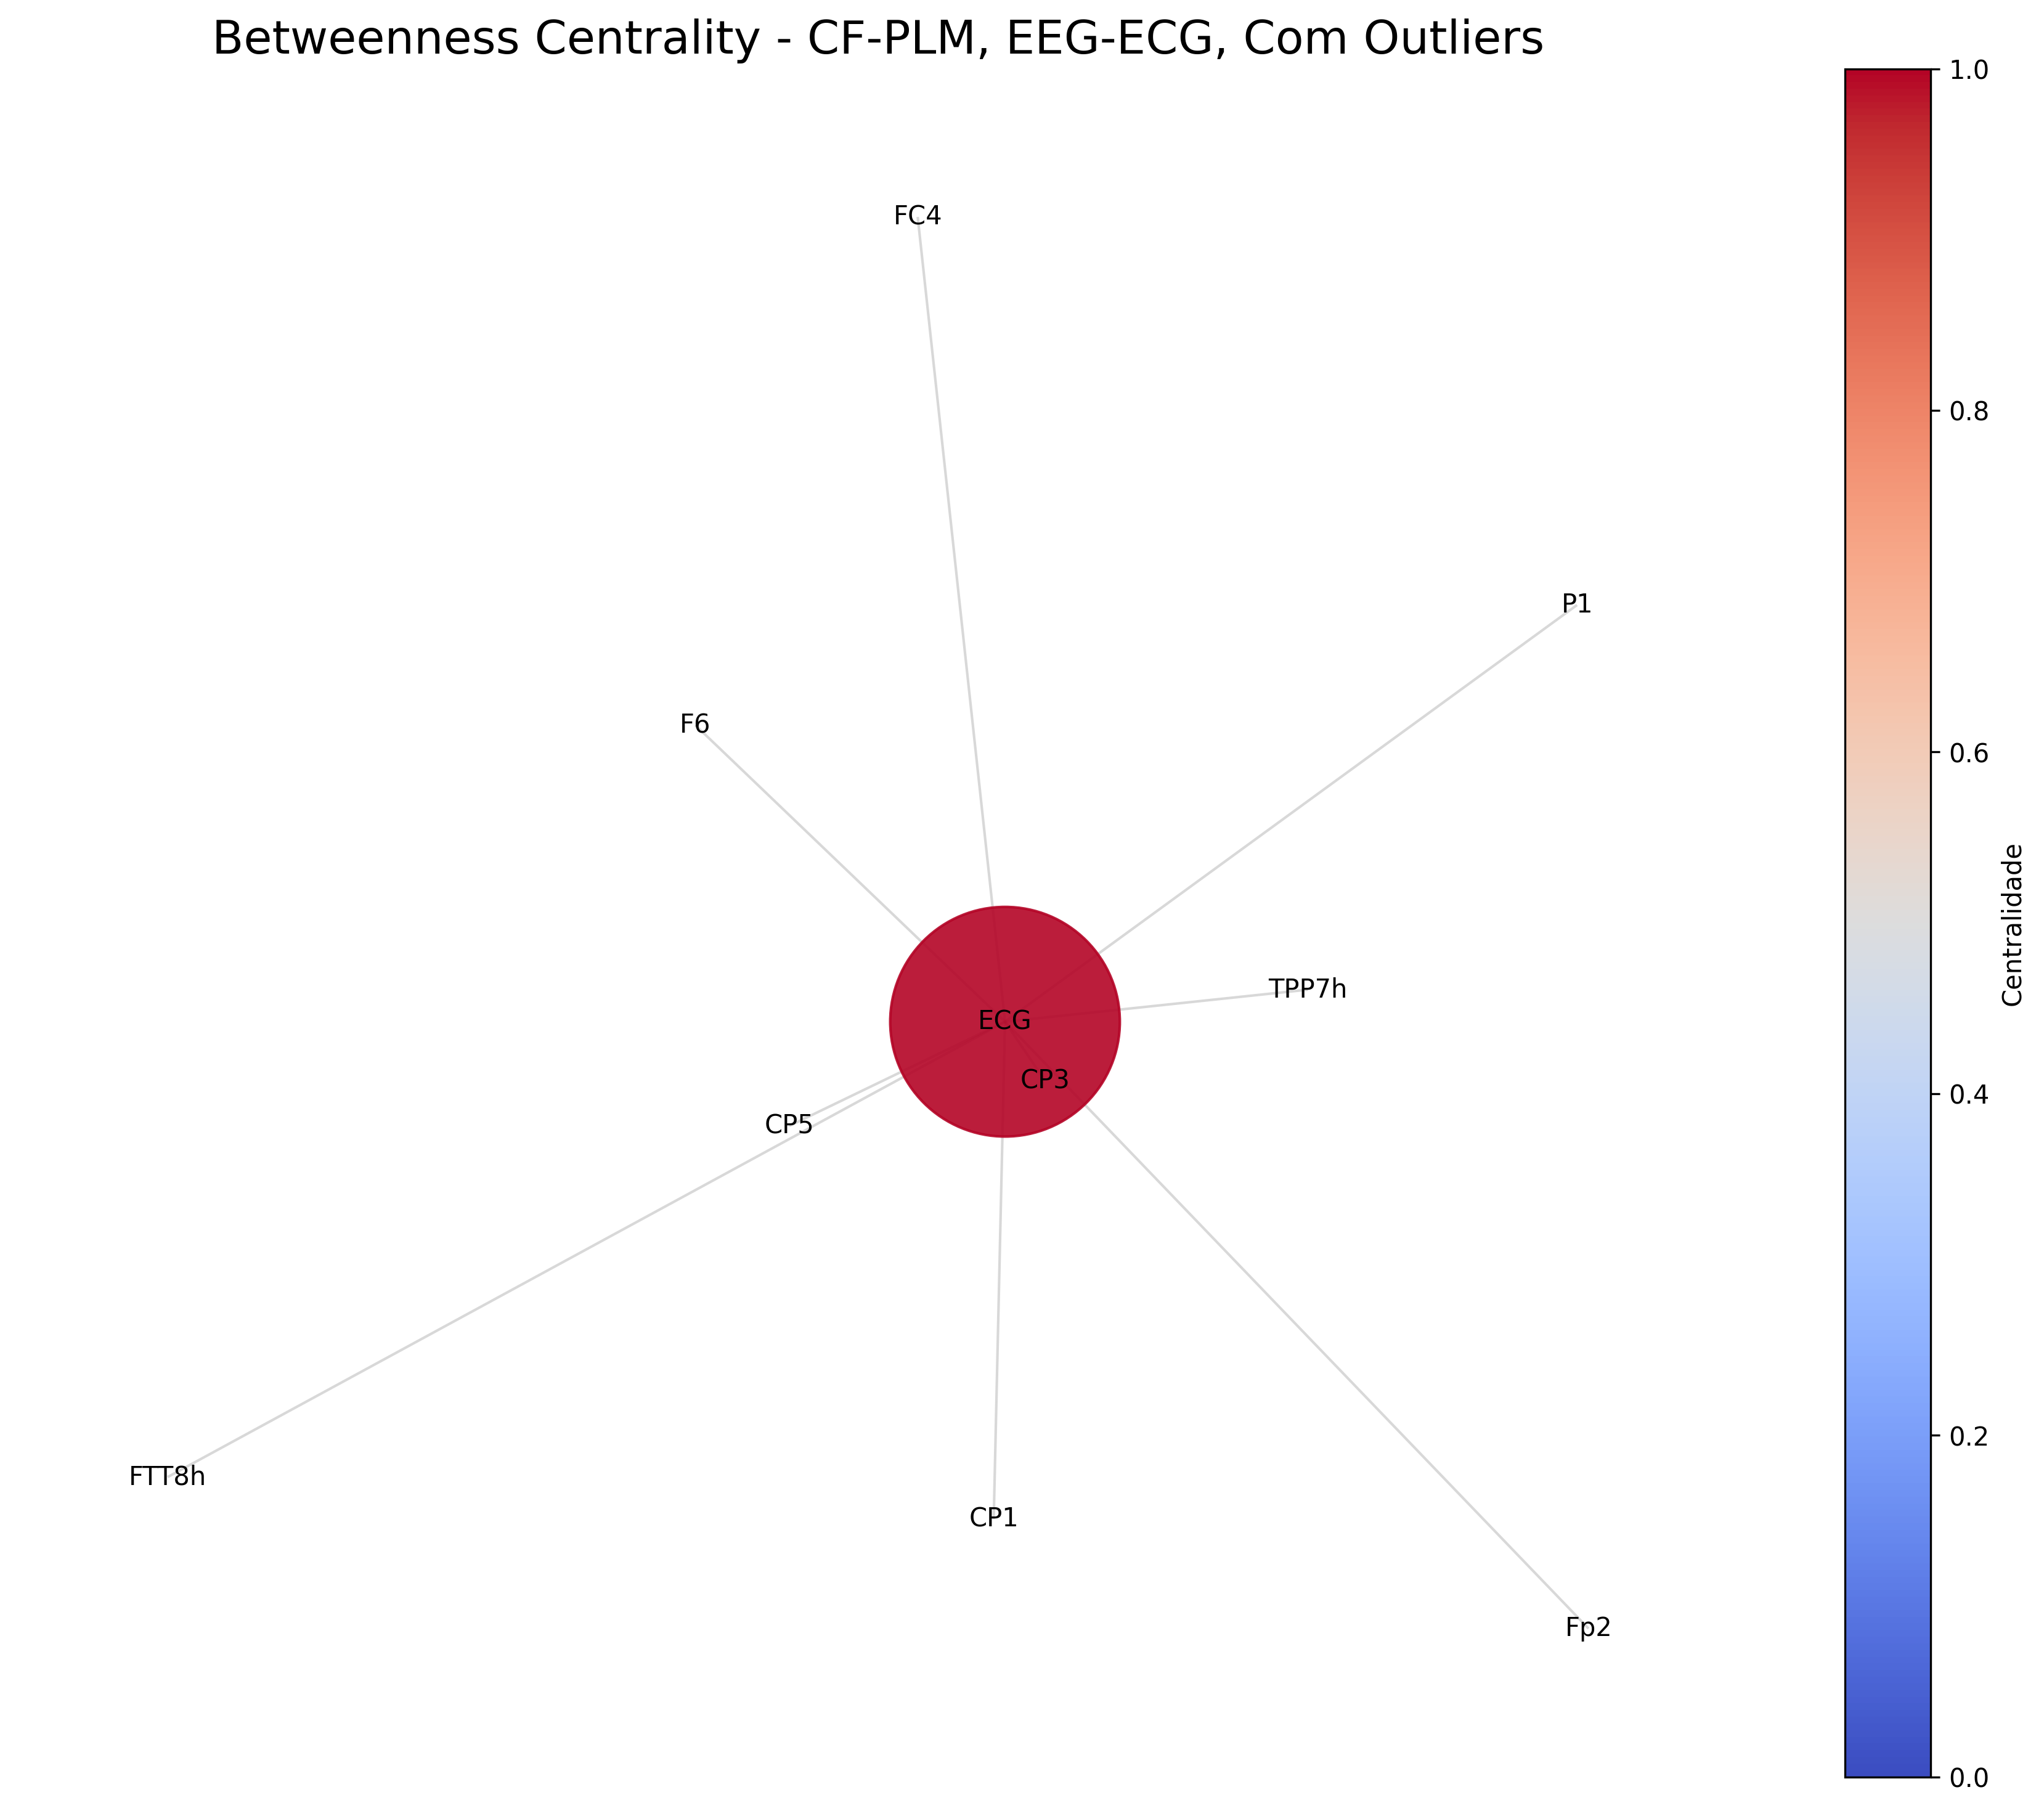
\includegraphics[width=0.45\textwidth]{figs/7_bootstrap_results_analysis/3_centrality_graphs/Betweenness_Centrality__CFPLM_EEGECG_Com_Outliers.png}
        \label{fig:bc_cfplm_eegecg_com}
    }
    \quad
    \subfloat[Sem Outliers]{
        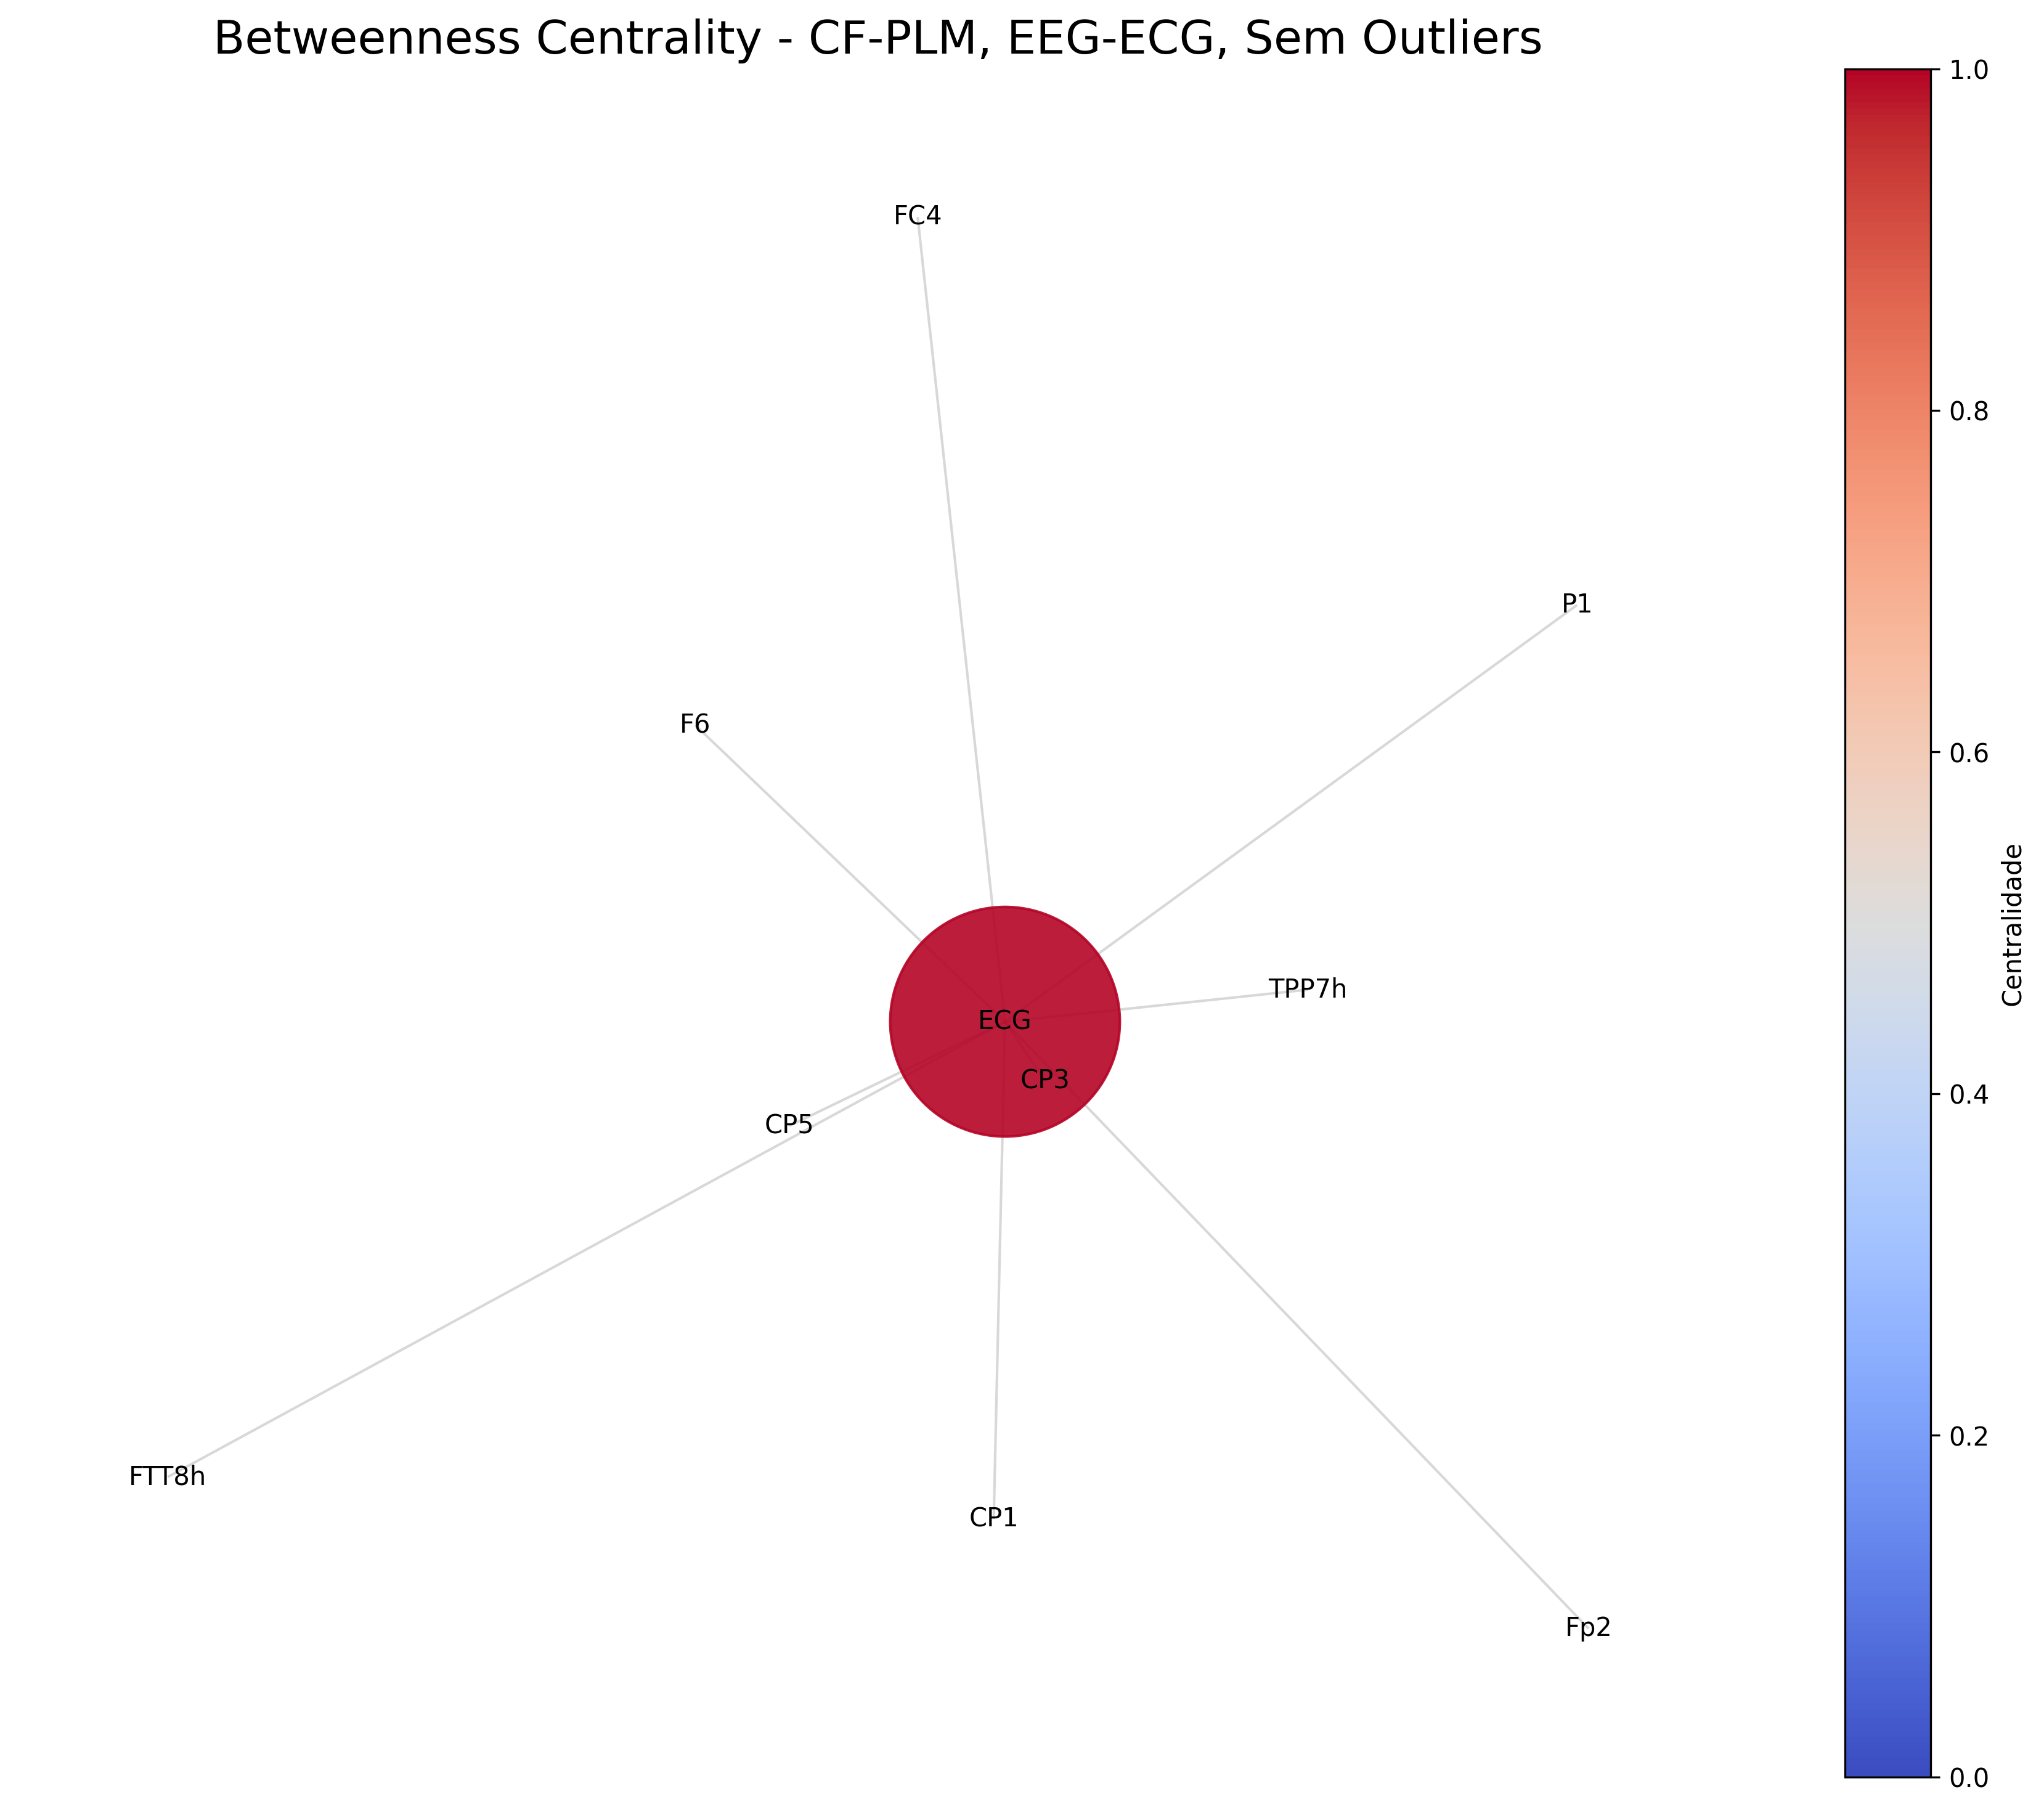
\includegraphics[width=0.45\textwidth]{figs/7_bootstrap_results_analysis/3_centrality_graphs/Betweenness_Centrality__CFPLM_EEGECG_Sem_Outliers.png}
        \label{fig:bc_cfplm_eegecg_sem}
    }
    \caption{Betweenness Centrality no cenário CF-PLM (EEG-ECG). O canal \emph{ECG} domina a rede em ambos os cenários.}
    \label{fig:bc_cfplm_eegecg}
\end{figure}

Nos gráficos da Figura~\ref{fig:bc_cfplm_eegecg}, o canal \emph{ECG} aparece como o nó com maior \emph{betweenness centrality}, pois todas as conexões \emph{cross-frequency} entre EEG e ECG precisam passar por ele. A remoção de outliers não altera substancialmente a estrutura: o \emph{ECG} continua central. Isso indica uma rede “estrela” em torno do canal cardíaco, coerente com a natureza do acoplamento \emph{cross-frequency} \cite{bullmore2009complex}.

\subsubsection{PLI (EEG-EEG)}
\begin{figure}[htb]
    \centering
    \subfloat[Com Outliers]{
        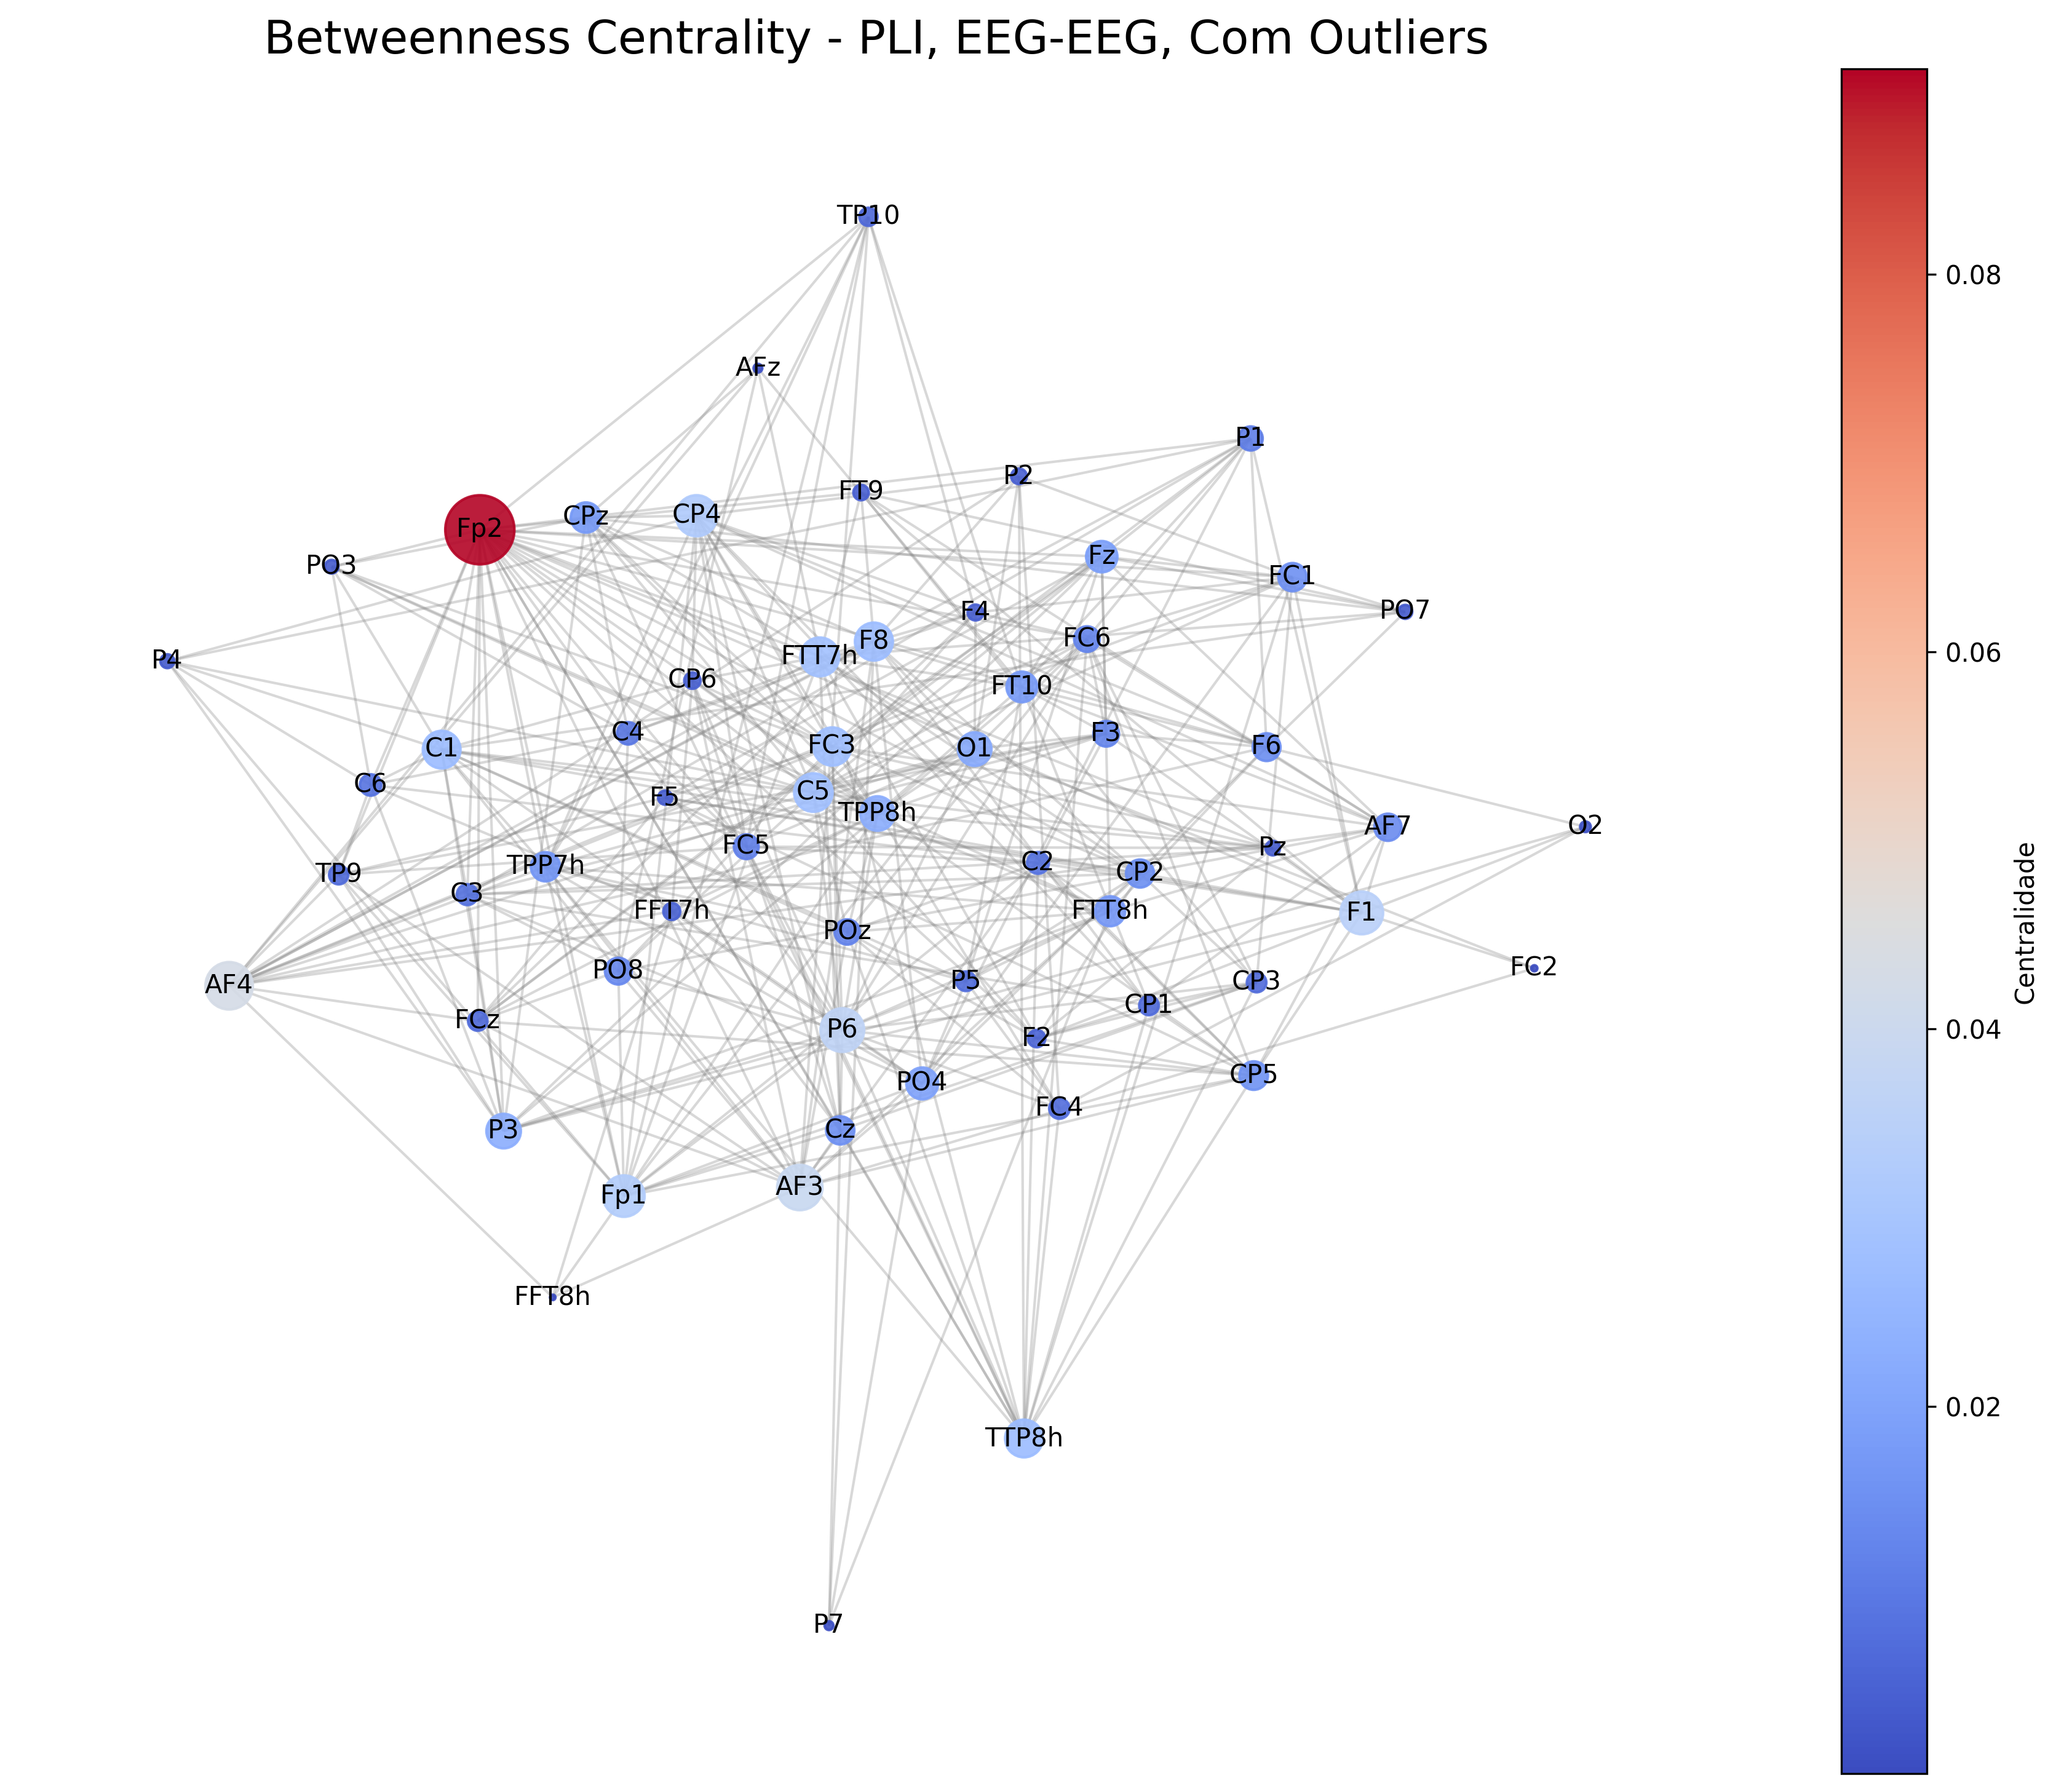
\includegraphics[width=0.45\textwidth]{figs/7_bootstrap_results_analysis/3_centrality_graphs/Betweenness_Centrality__PLI_EEGEEG_Com_Outliers.png}
        \label{fig:bc_pli_eegeeg_com}
    }
    \quad
    \subfloat[Sem Outliers]{
        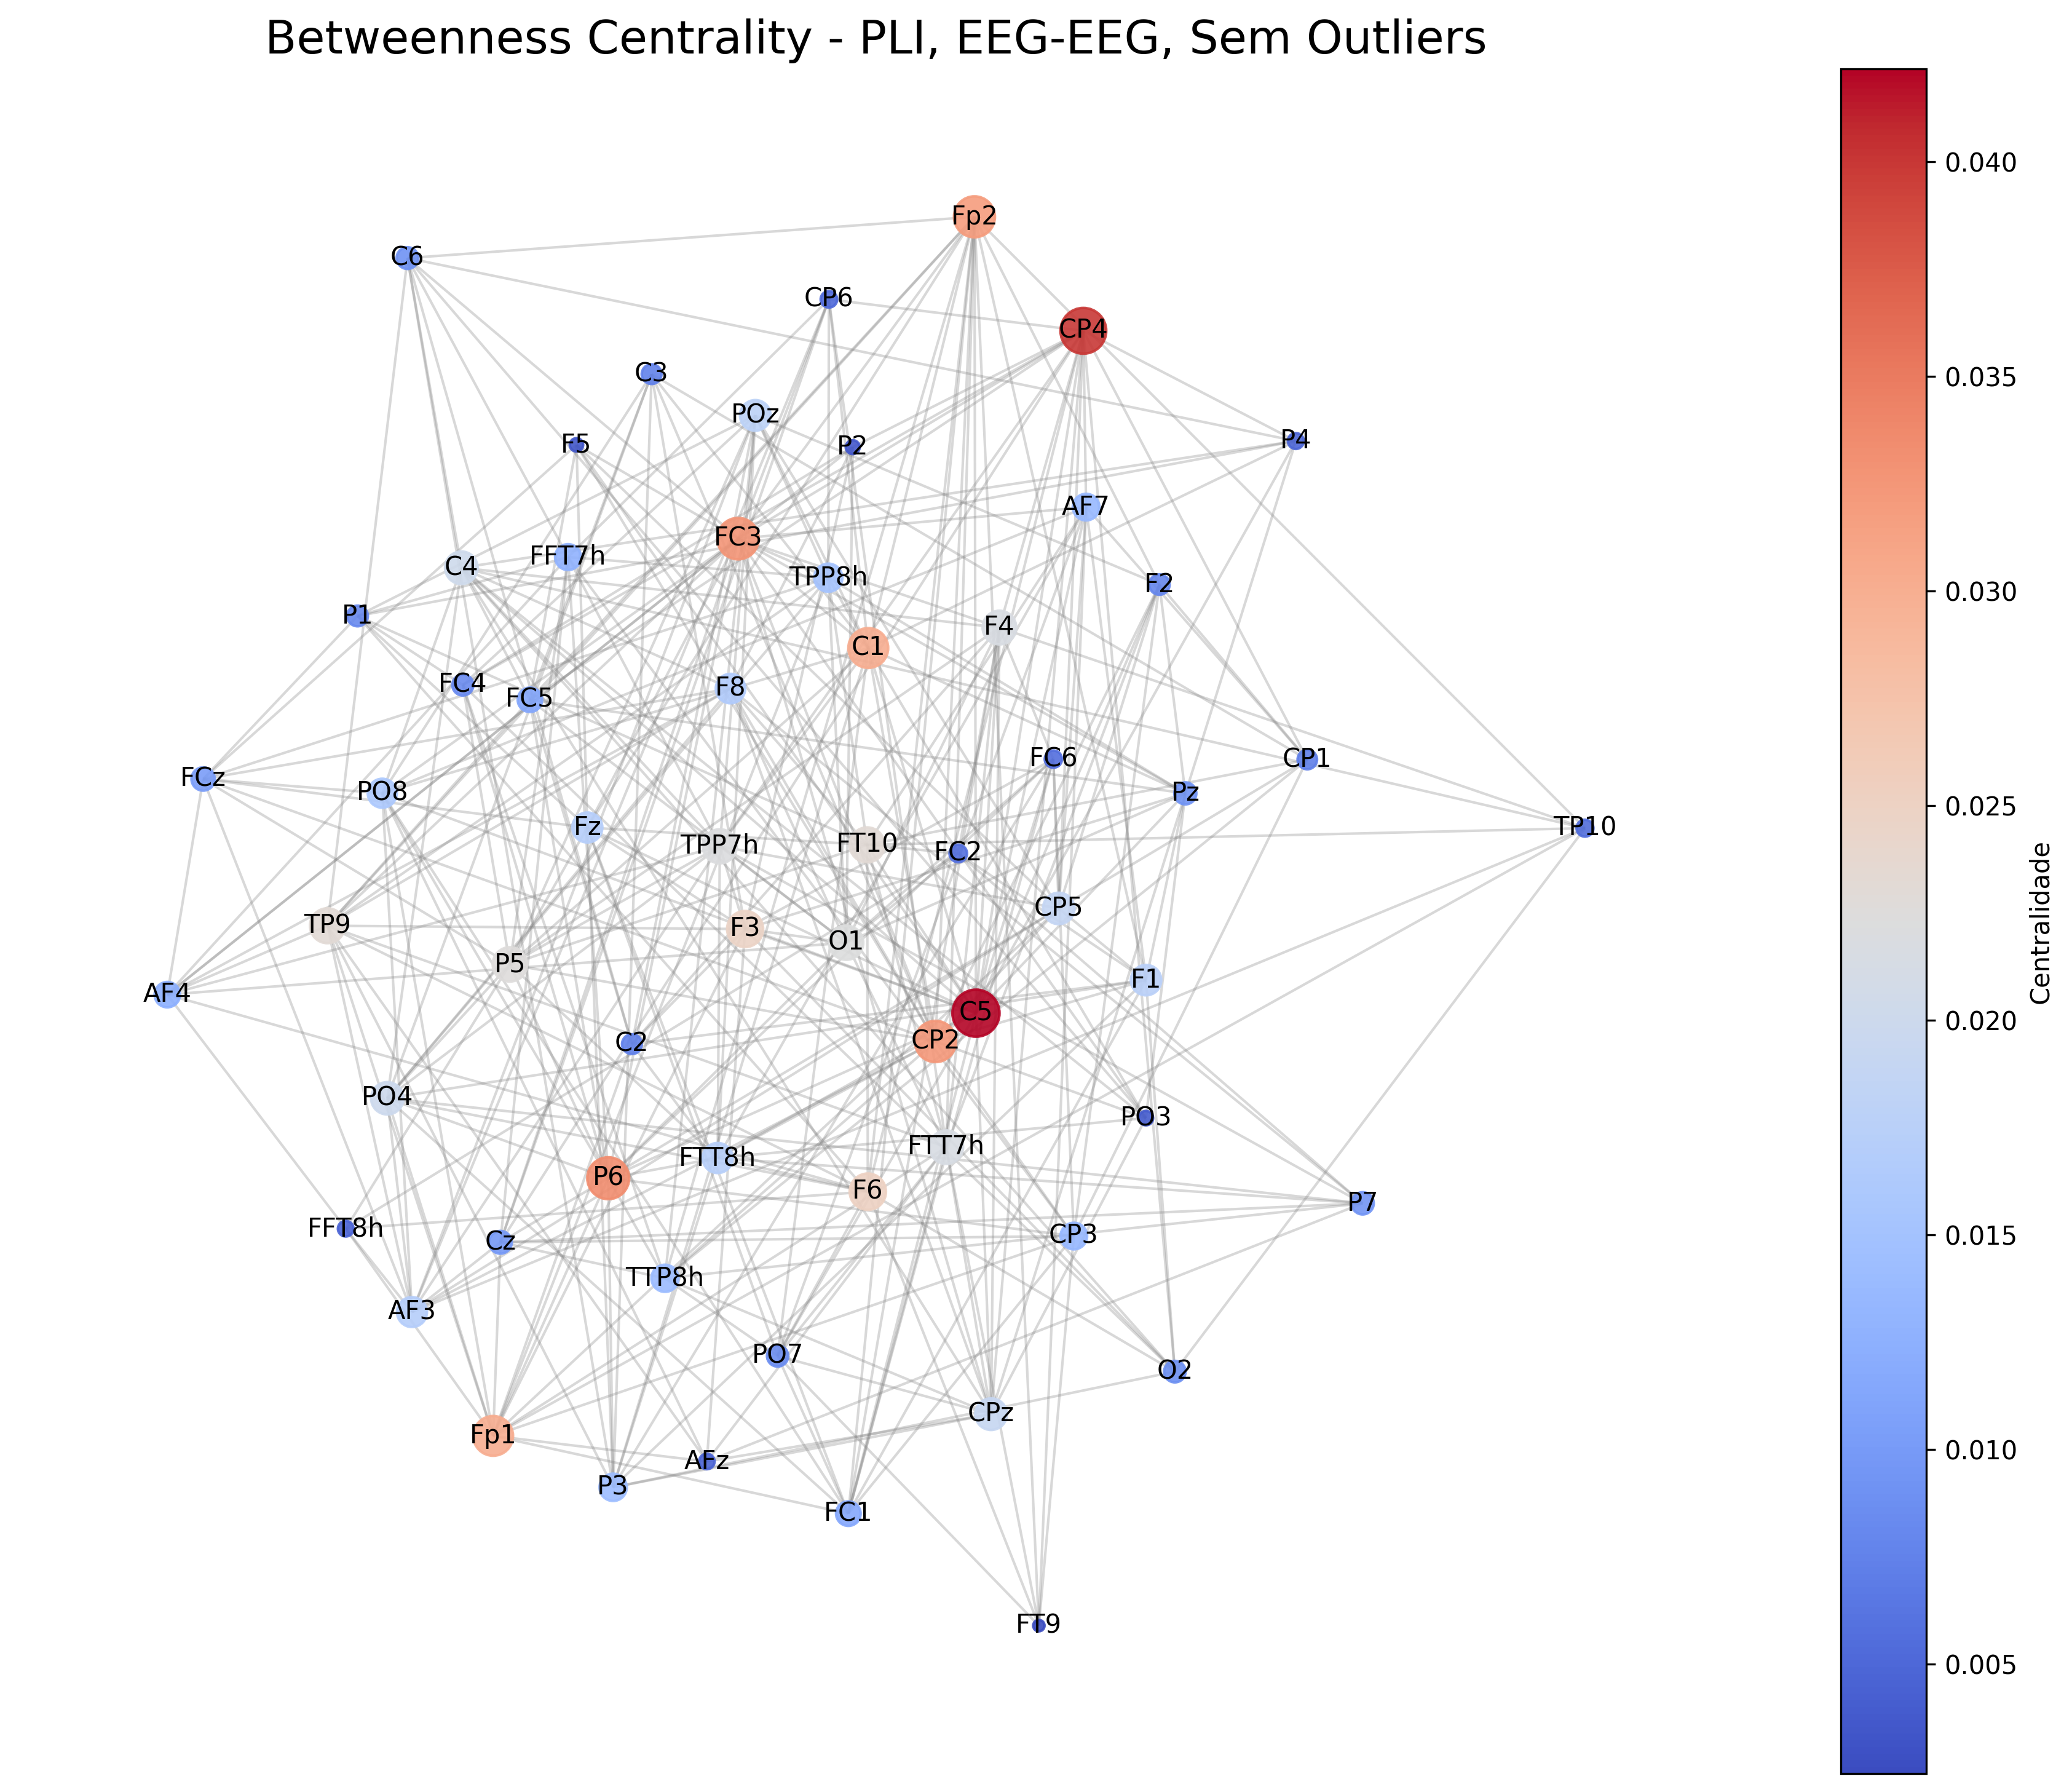
\includegraphics[width=0.45\textwidth]{figs/7_bootstrap_results_analysis/3_centrality_graphs/Betweenness_Centrality__PLI_EEGEEG_Sem_Outliers.png}
        \label{fig:bc_pli_eegeeg_sem}
    }
    \caption{Betweenness Centrality no cenário PLI (EEG-EEG). Canais frontais ou parietais podem se destacar como “pontes” de sincronização.}
    \label{fig:bc_pli_eegeeg}
\end{figure}

Na Figura~\ref{fig:bc_pli_eegeeg}, observa-se uma rede EEG-EEG mais complexa, em que certos canais (por exemplo, Fp2, CP2) exibem maior \emph{betweenness centrality} e atuam como “pontes” para muitas conexões. A remoção de outliers não altera de forma drástica os canais centrais, sugerindo que as conexões mais fortes (e que envolvem rotas essenciais) permanecem estáveis. Canais frontais ou parietais com alta centralidade podem refletir regiões-chave na sincronização de fase iso-frequencial \cite{rubinov2010complex}.

\subsection{Degree Centrality}
A \emph{degree centrality} contabiliza o número de conexões diretas de cada nó, medindo sua “popularidade” na rede. Um canal com alto grau possui mais conexões do que os demais \cite{newman2010networks}.

\subsubsection{CF-PLM (EEG-ECG)}
\begin{figure}[htb]
    \centering
    \subfloat[Com Outliers]{
        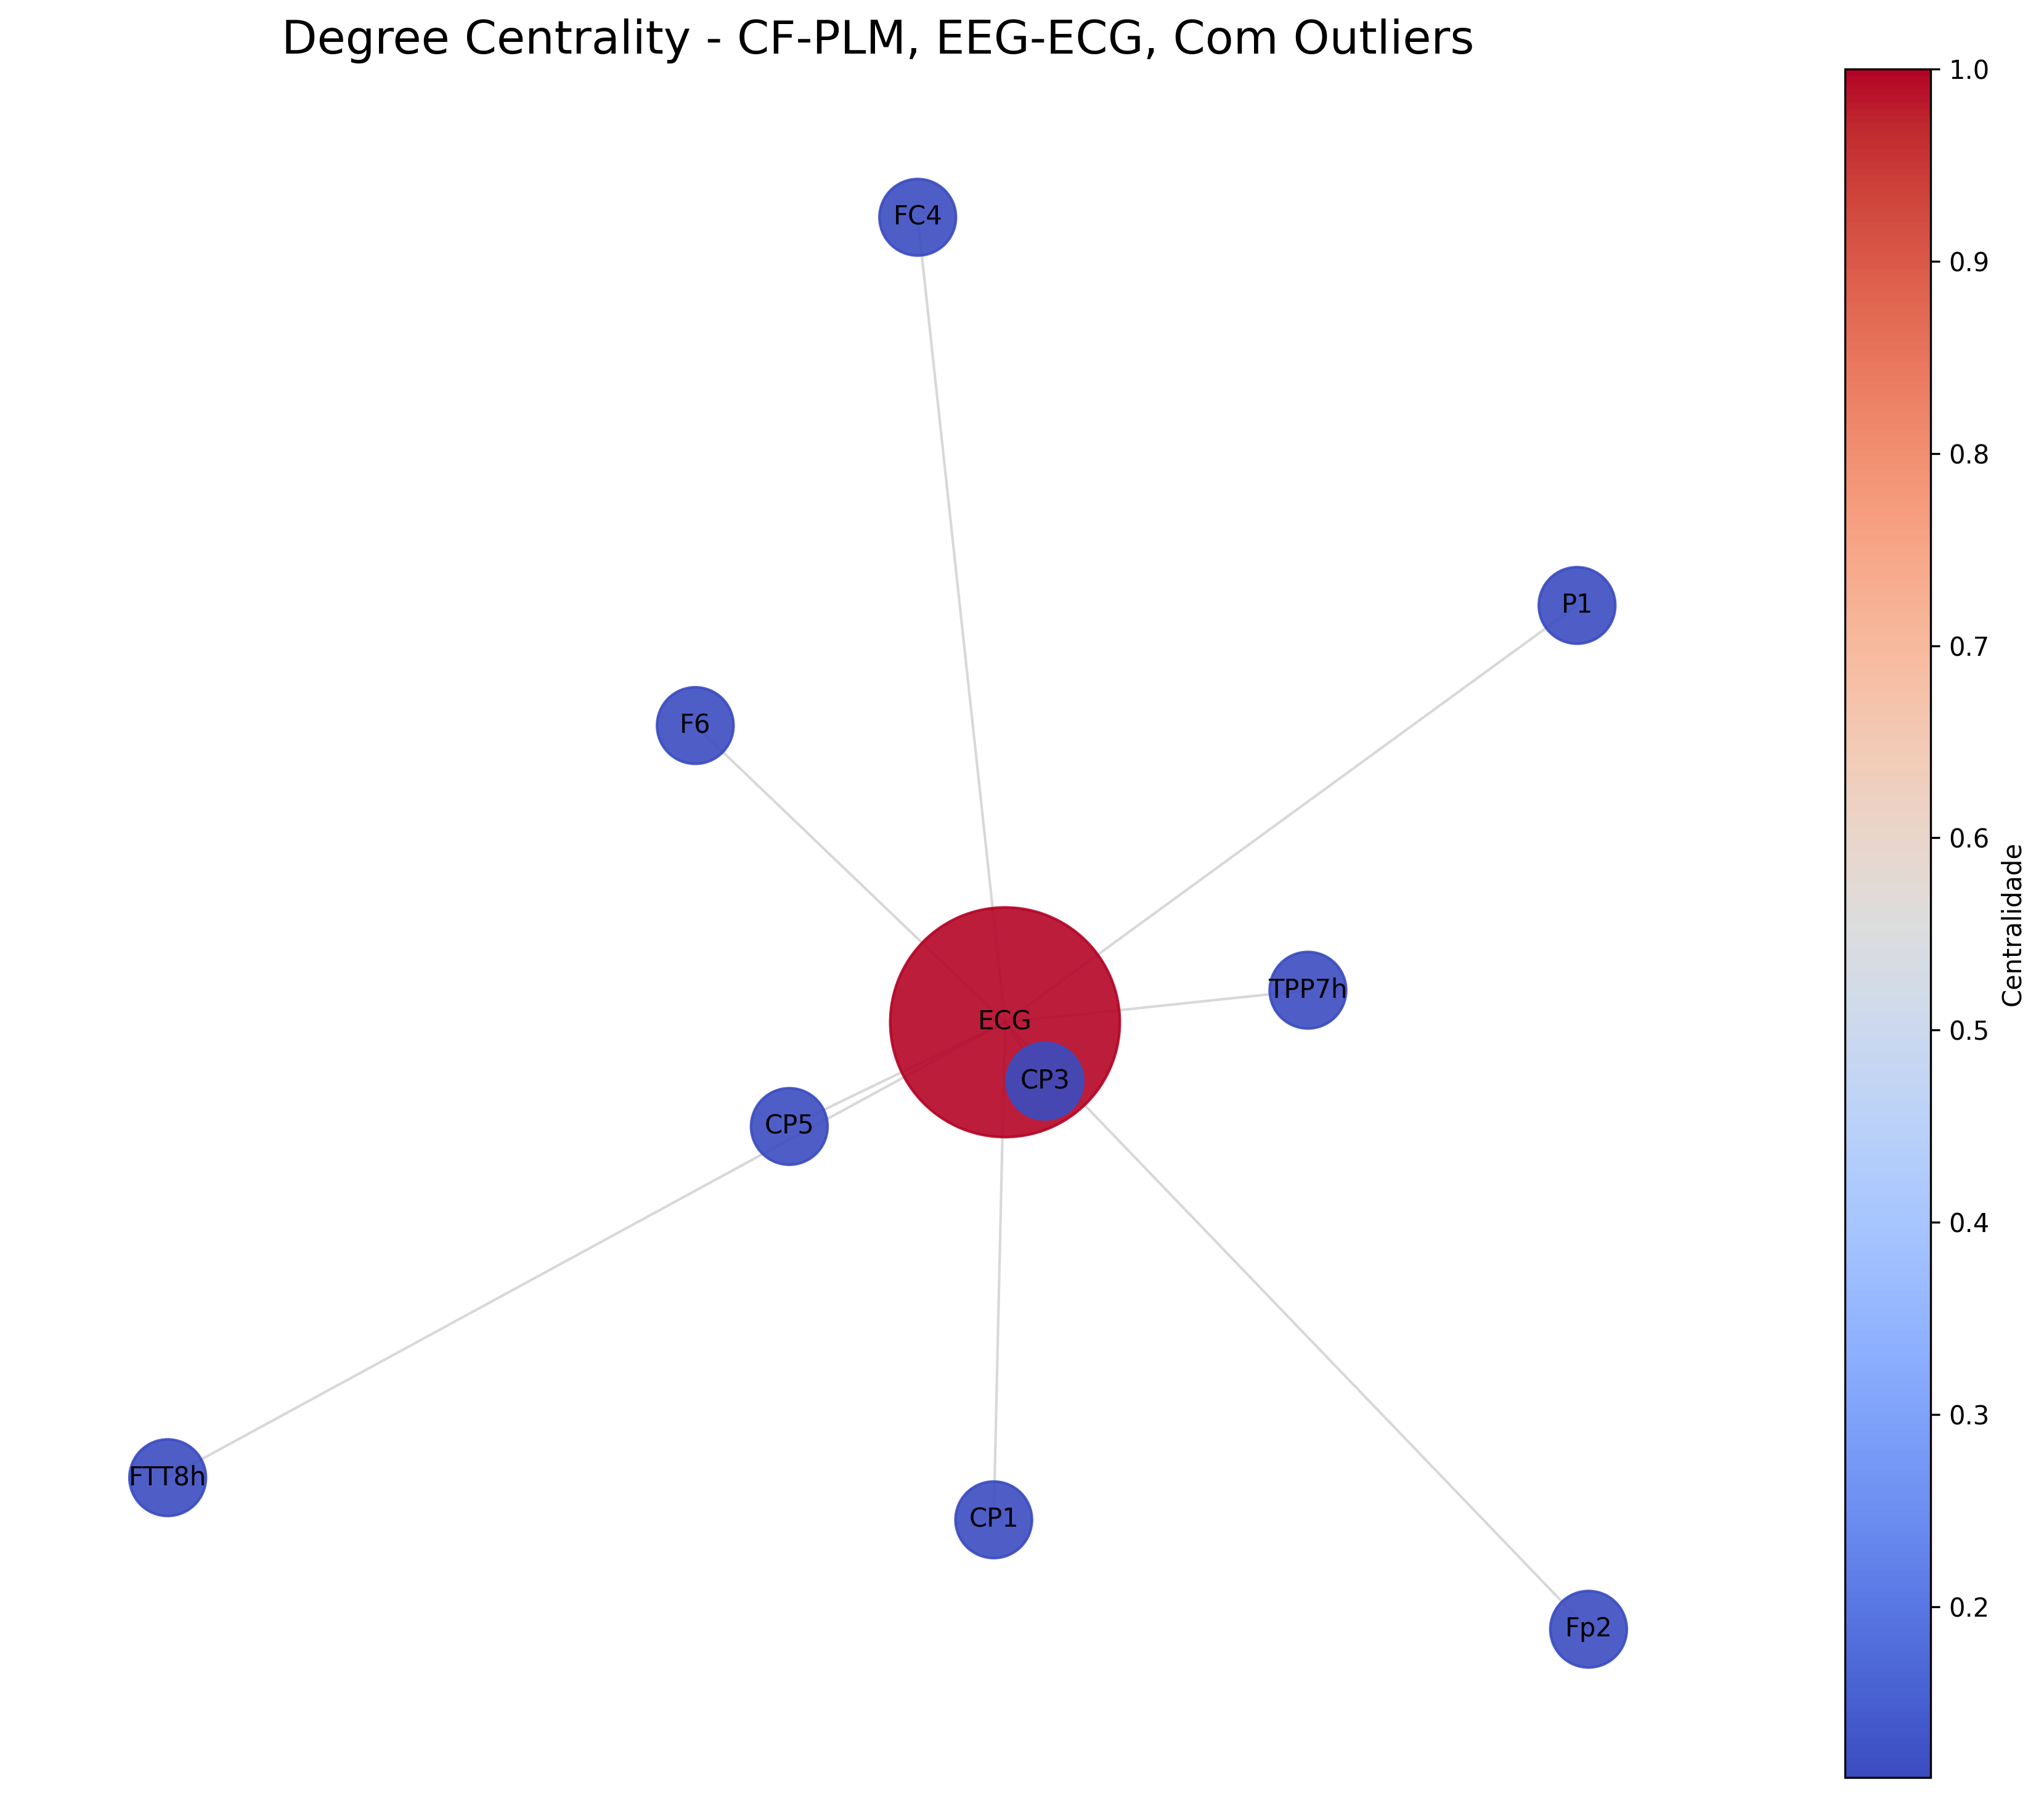
\includegraphics[width=0.45\textwidth]{figs/7_bootstrap_results_analysis/3_centrality_graphs/Degree_Centrality__CFPLM_EEGECG_Com_Outliers.png}
        \label{fig:dc_cfplm_eegecg_com}
    }
    \quad
    \subfloat[Sem Outliers]{
        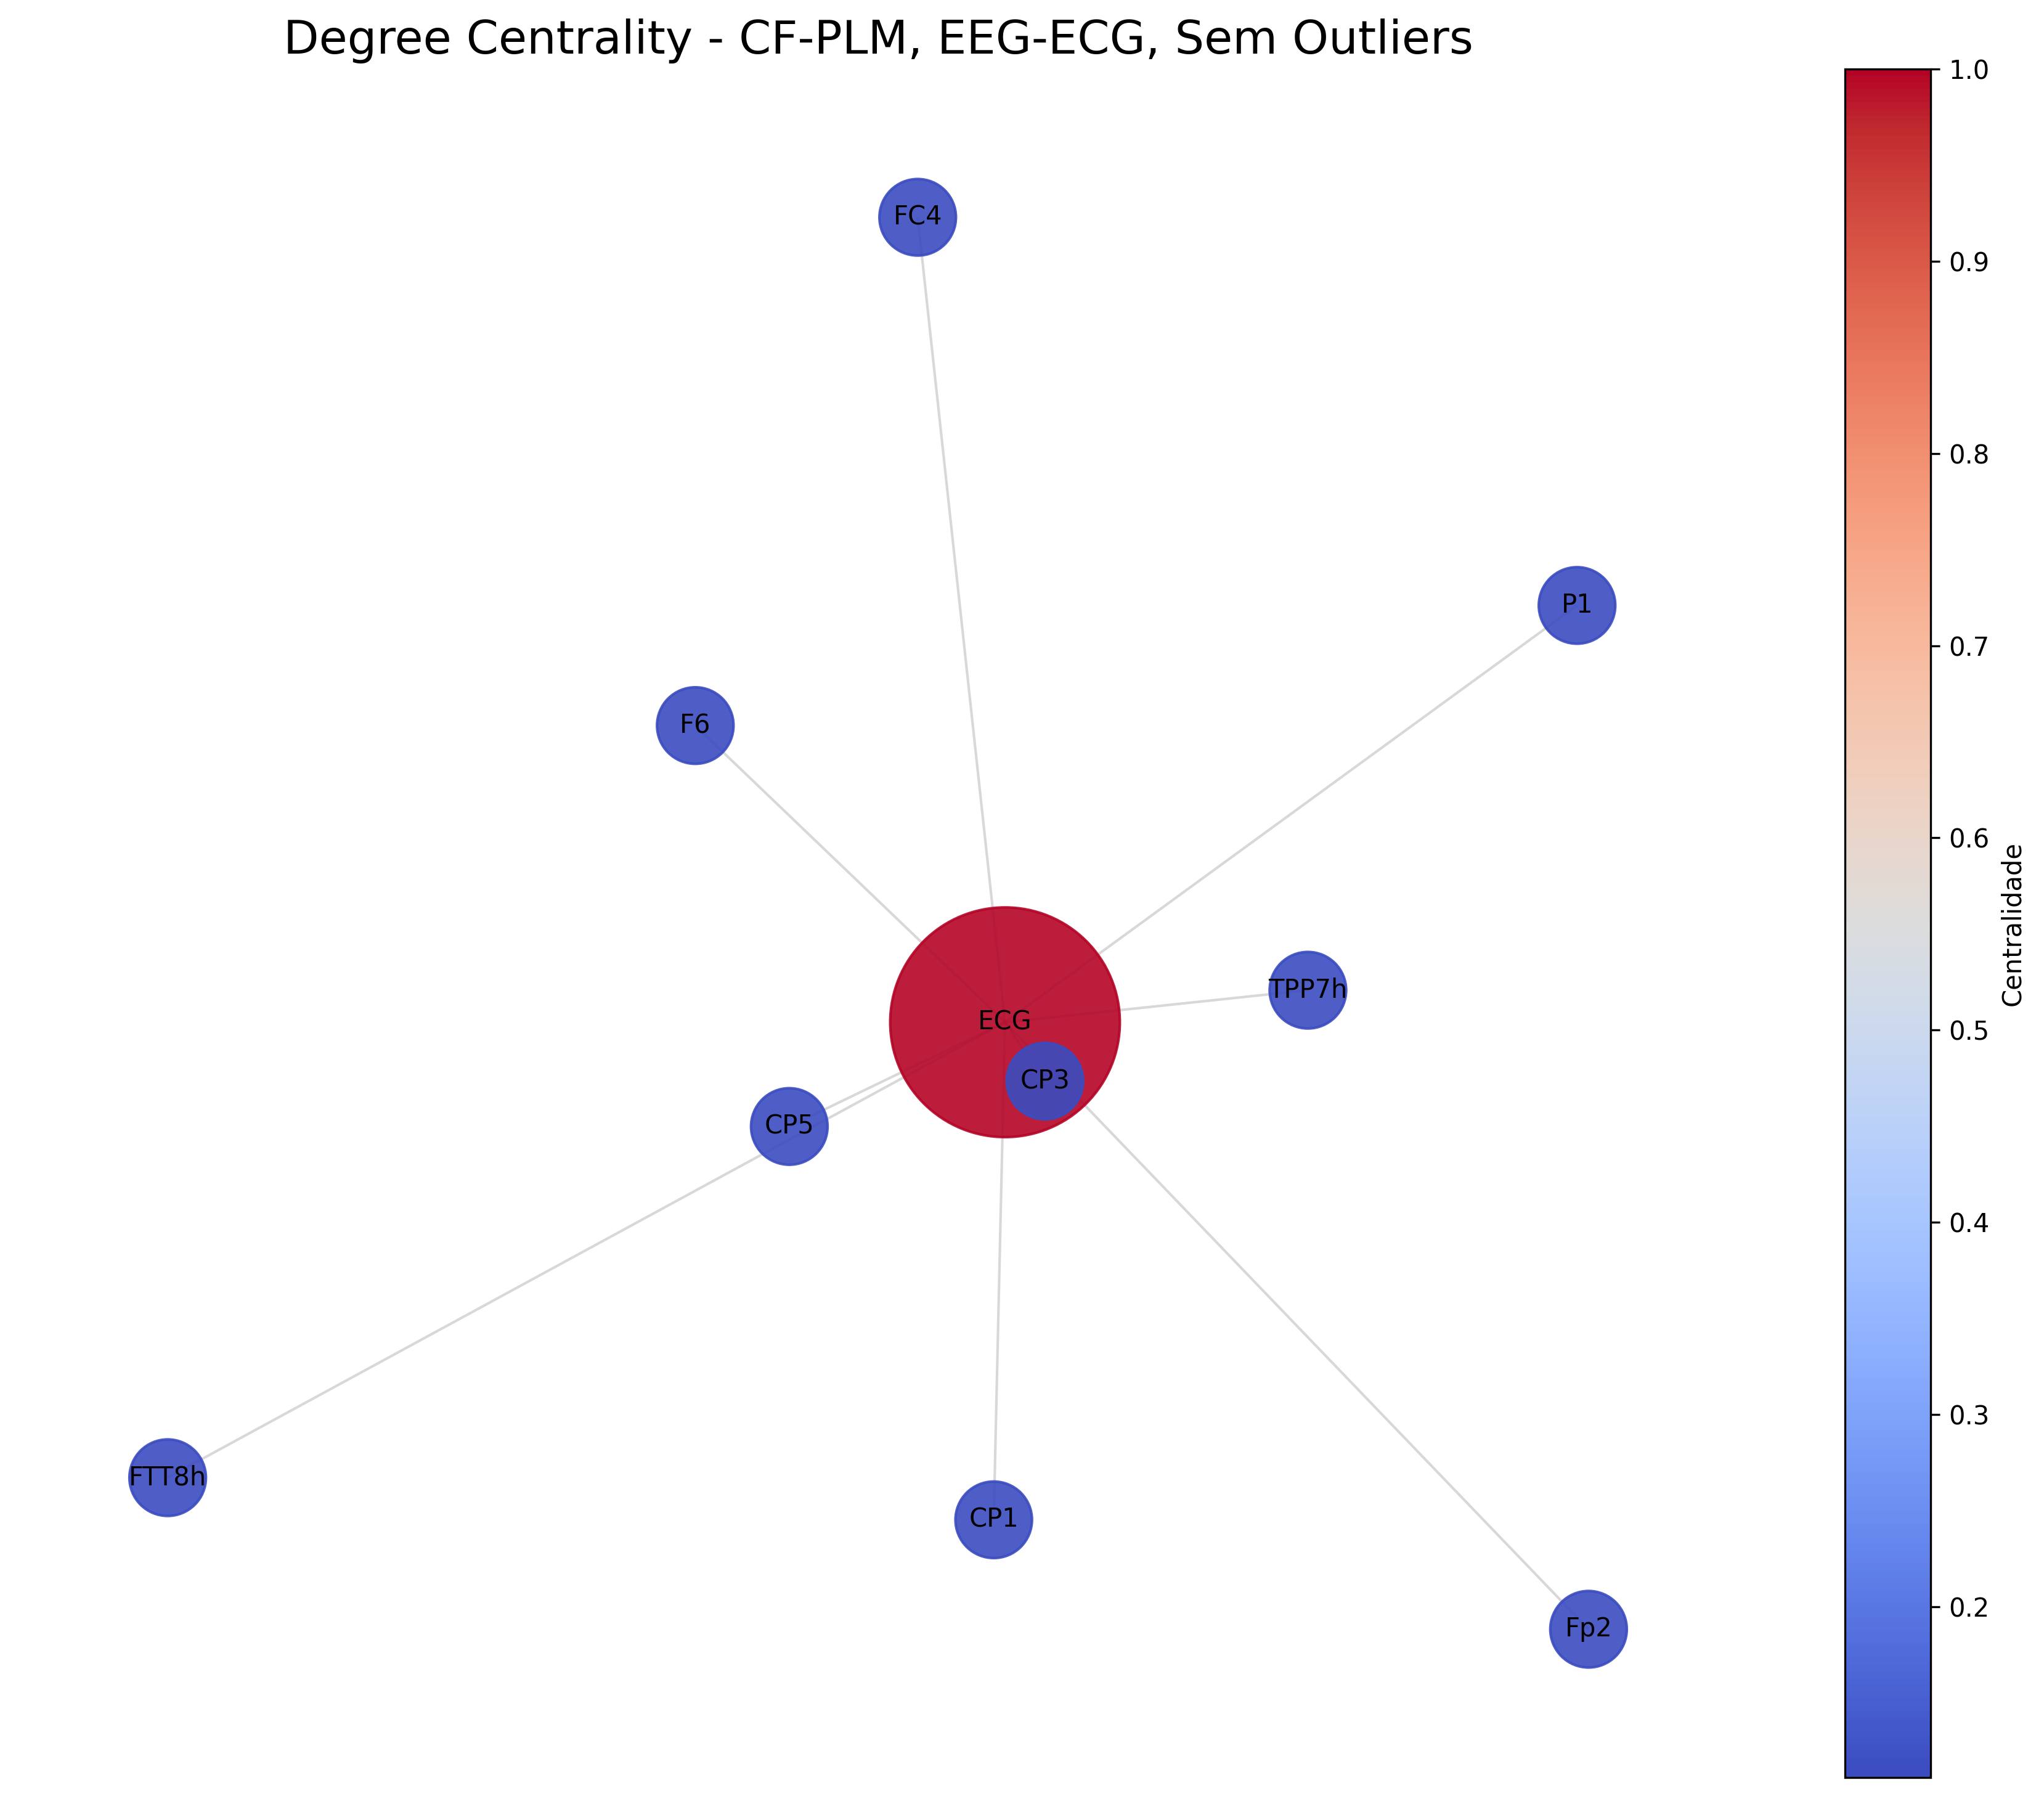
\includegraphics[width=0.45\textwidth]{figs/7_bootstrap_results_analysis/3_centrality_graphs/Degree_Centrality__CFPLM_EEGECG_Sem_Outliers.png}
        \label{fig:dc_cfplm_eegecg_sem}
    }
    \caption{Degree Centrality no cenário CF-PLM (EEG-ECG). O canal \emph{ECG} mantém o grau mais alto em ambos os cenários.}
    \label{fig:dc_cfplm_eegecg}
\end{figure}

Na Figura~\ref{fig:dc_cfplm_eegecg}, o \emph{ECG} novamente domina a rede com o maior grau, pois é o único canal cardíaco e qualquer conexão cross-frequency EEG-ECG passa por ele. Assim, todos os canais EEG conectados ao \emph{ECG} elevam seu grau, mas o \emph{ECG} concentra a maior parte das conexões diretas \cite{rubinov2010complex}. A remoção de outliers não muda essa hierarquia.

\subsubsection{PLI (EEG-EEG)}
\begin{figure}[htb]
    \centering
    \subfloat[Com Outliers]{
        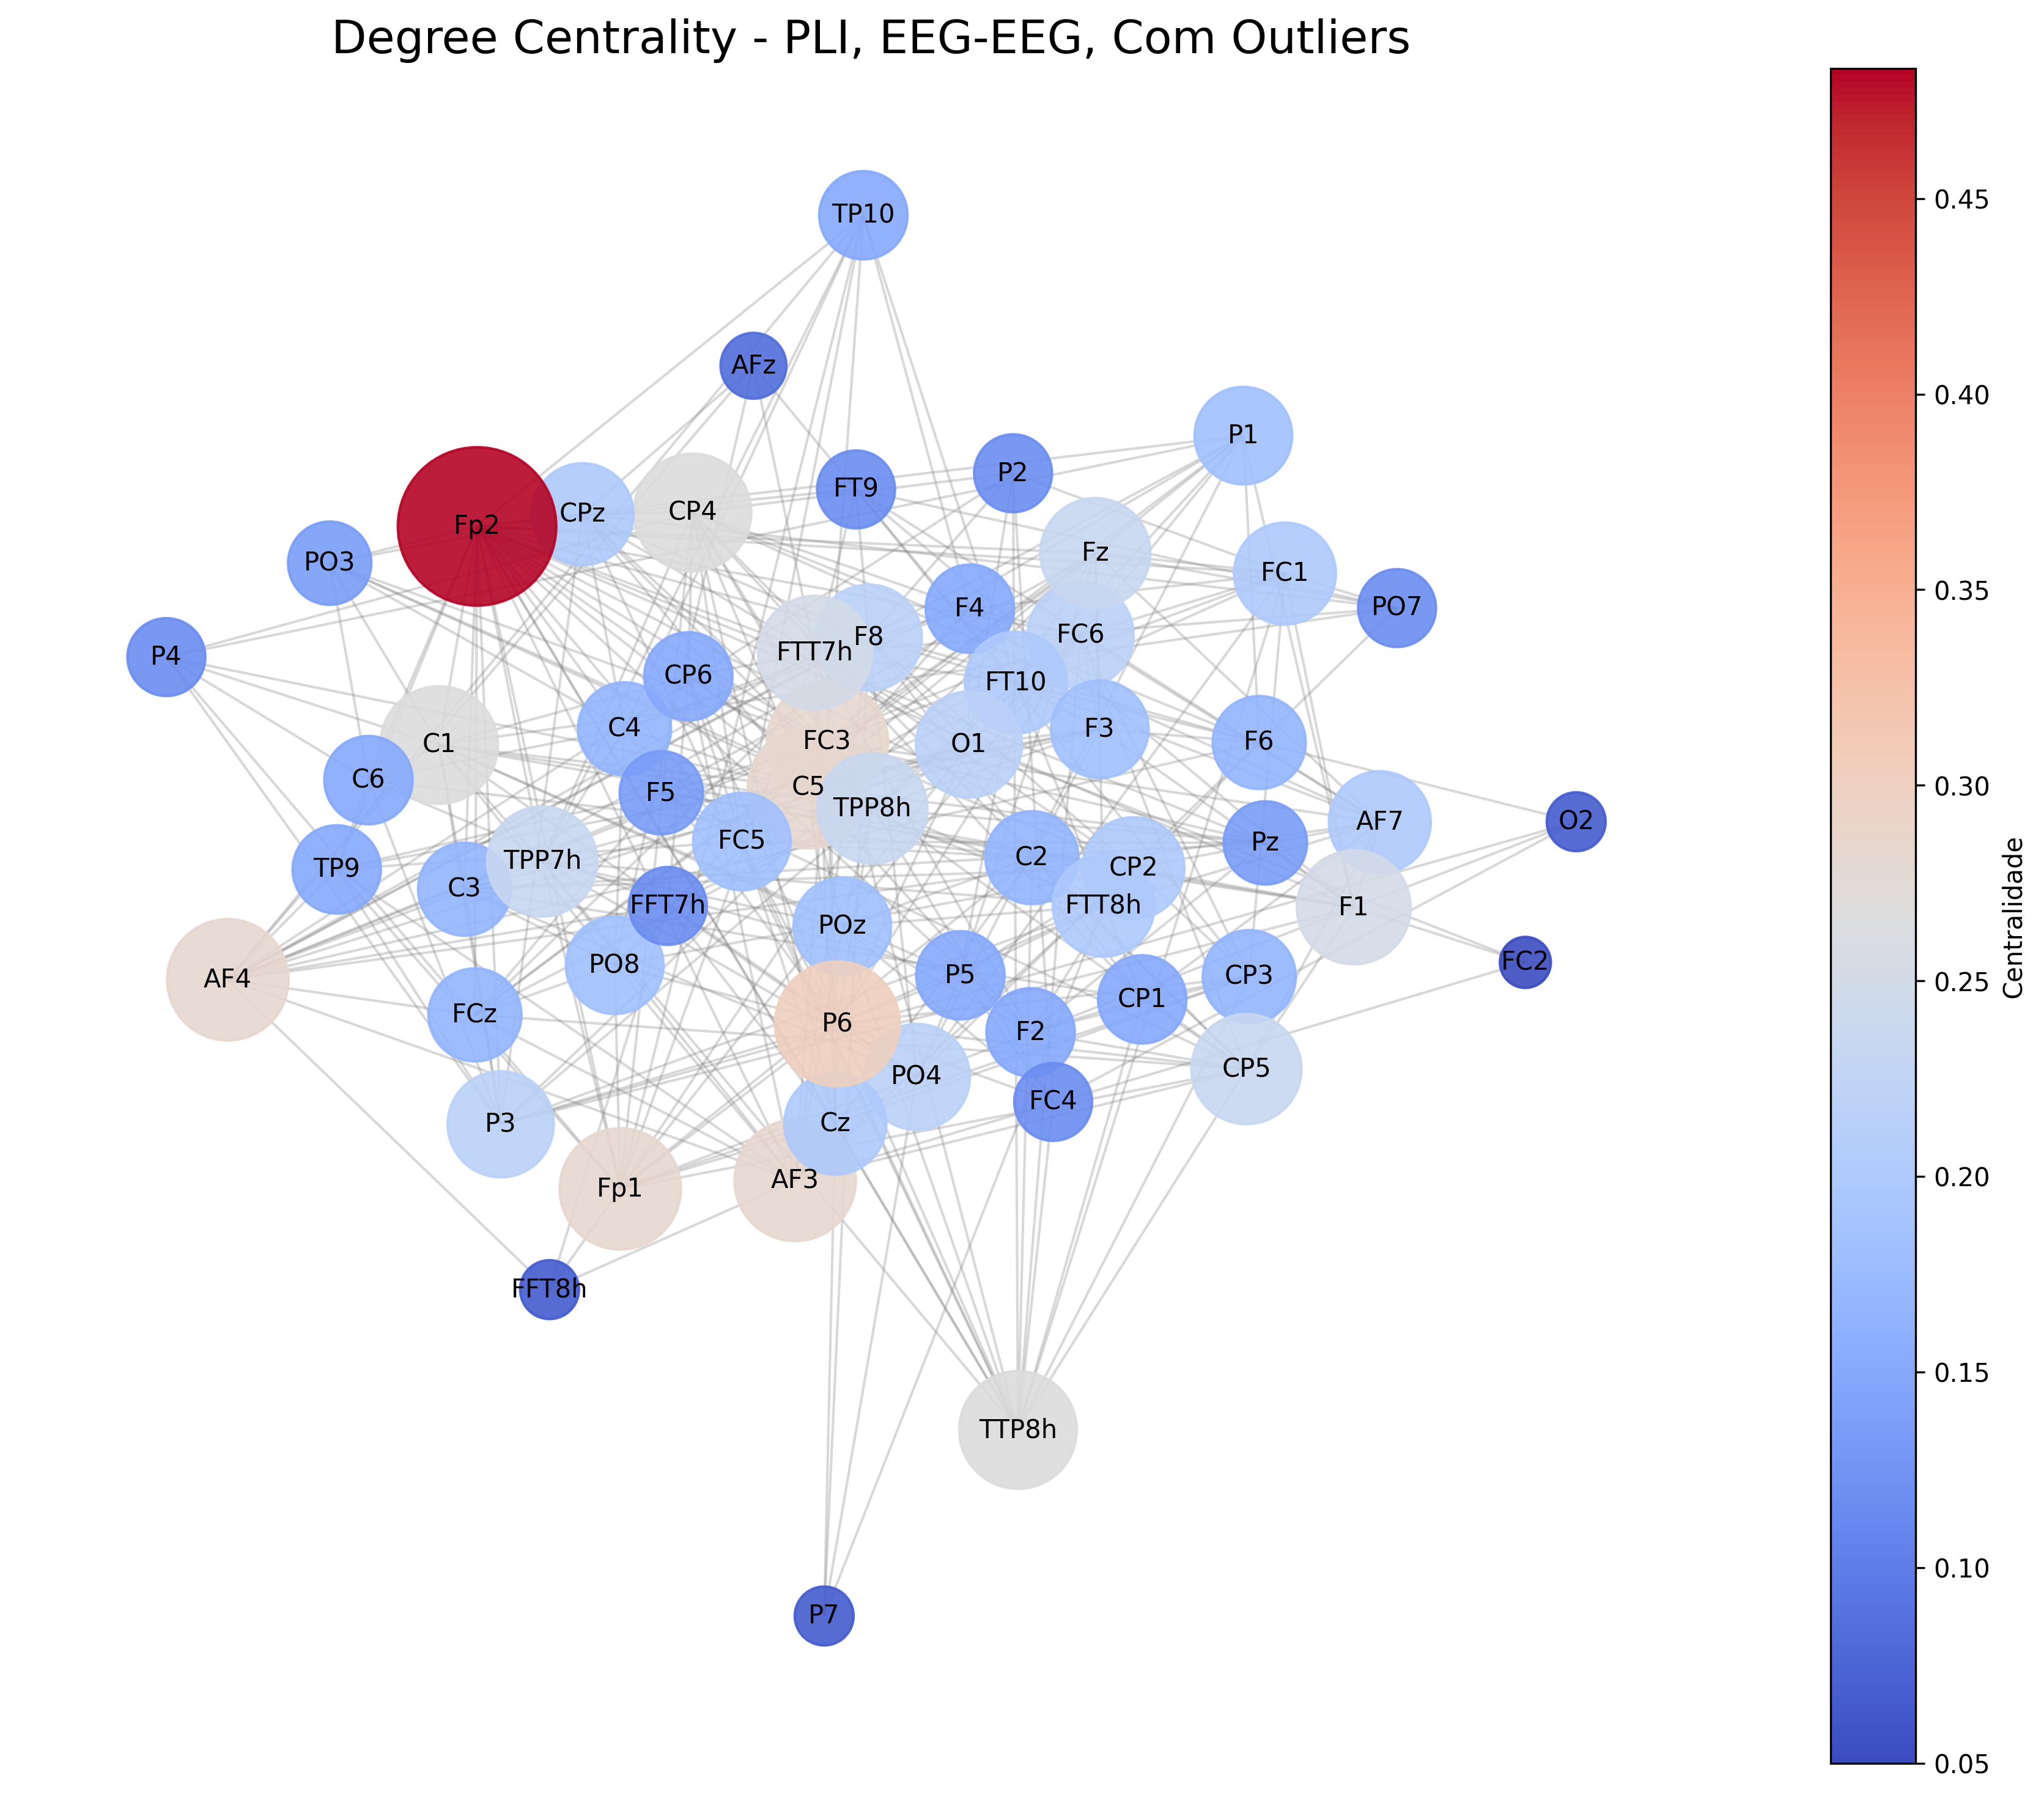
\includegraphics[width=0.45\textwidth]{figs/7_bootstrap_results_analysis/3_centrality_graphs/Degree_Centrality__PLI_EEGEEG_Com_Outliers.png}
        \label{fig:dc_pli_eegeeg_com}
    }
    \quad
    \subfloat[Sem Outliers]{
        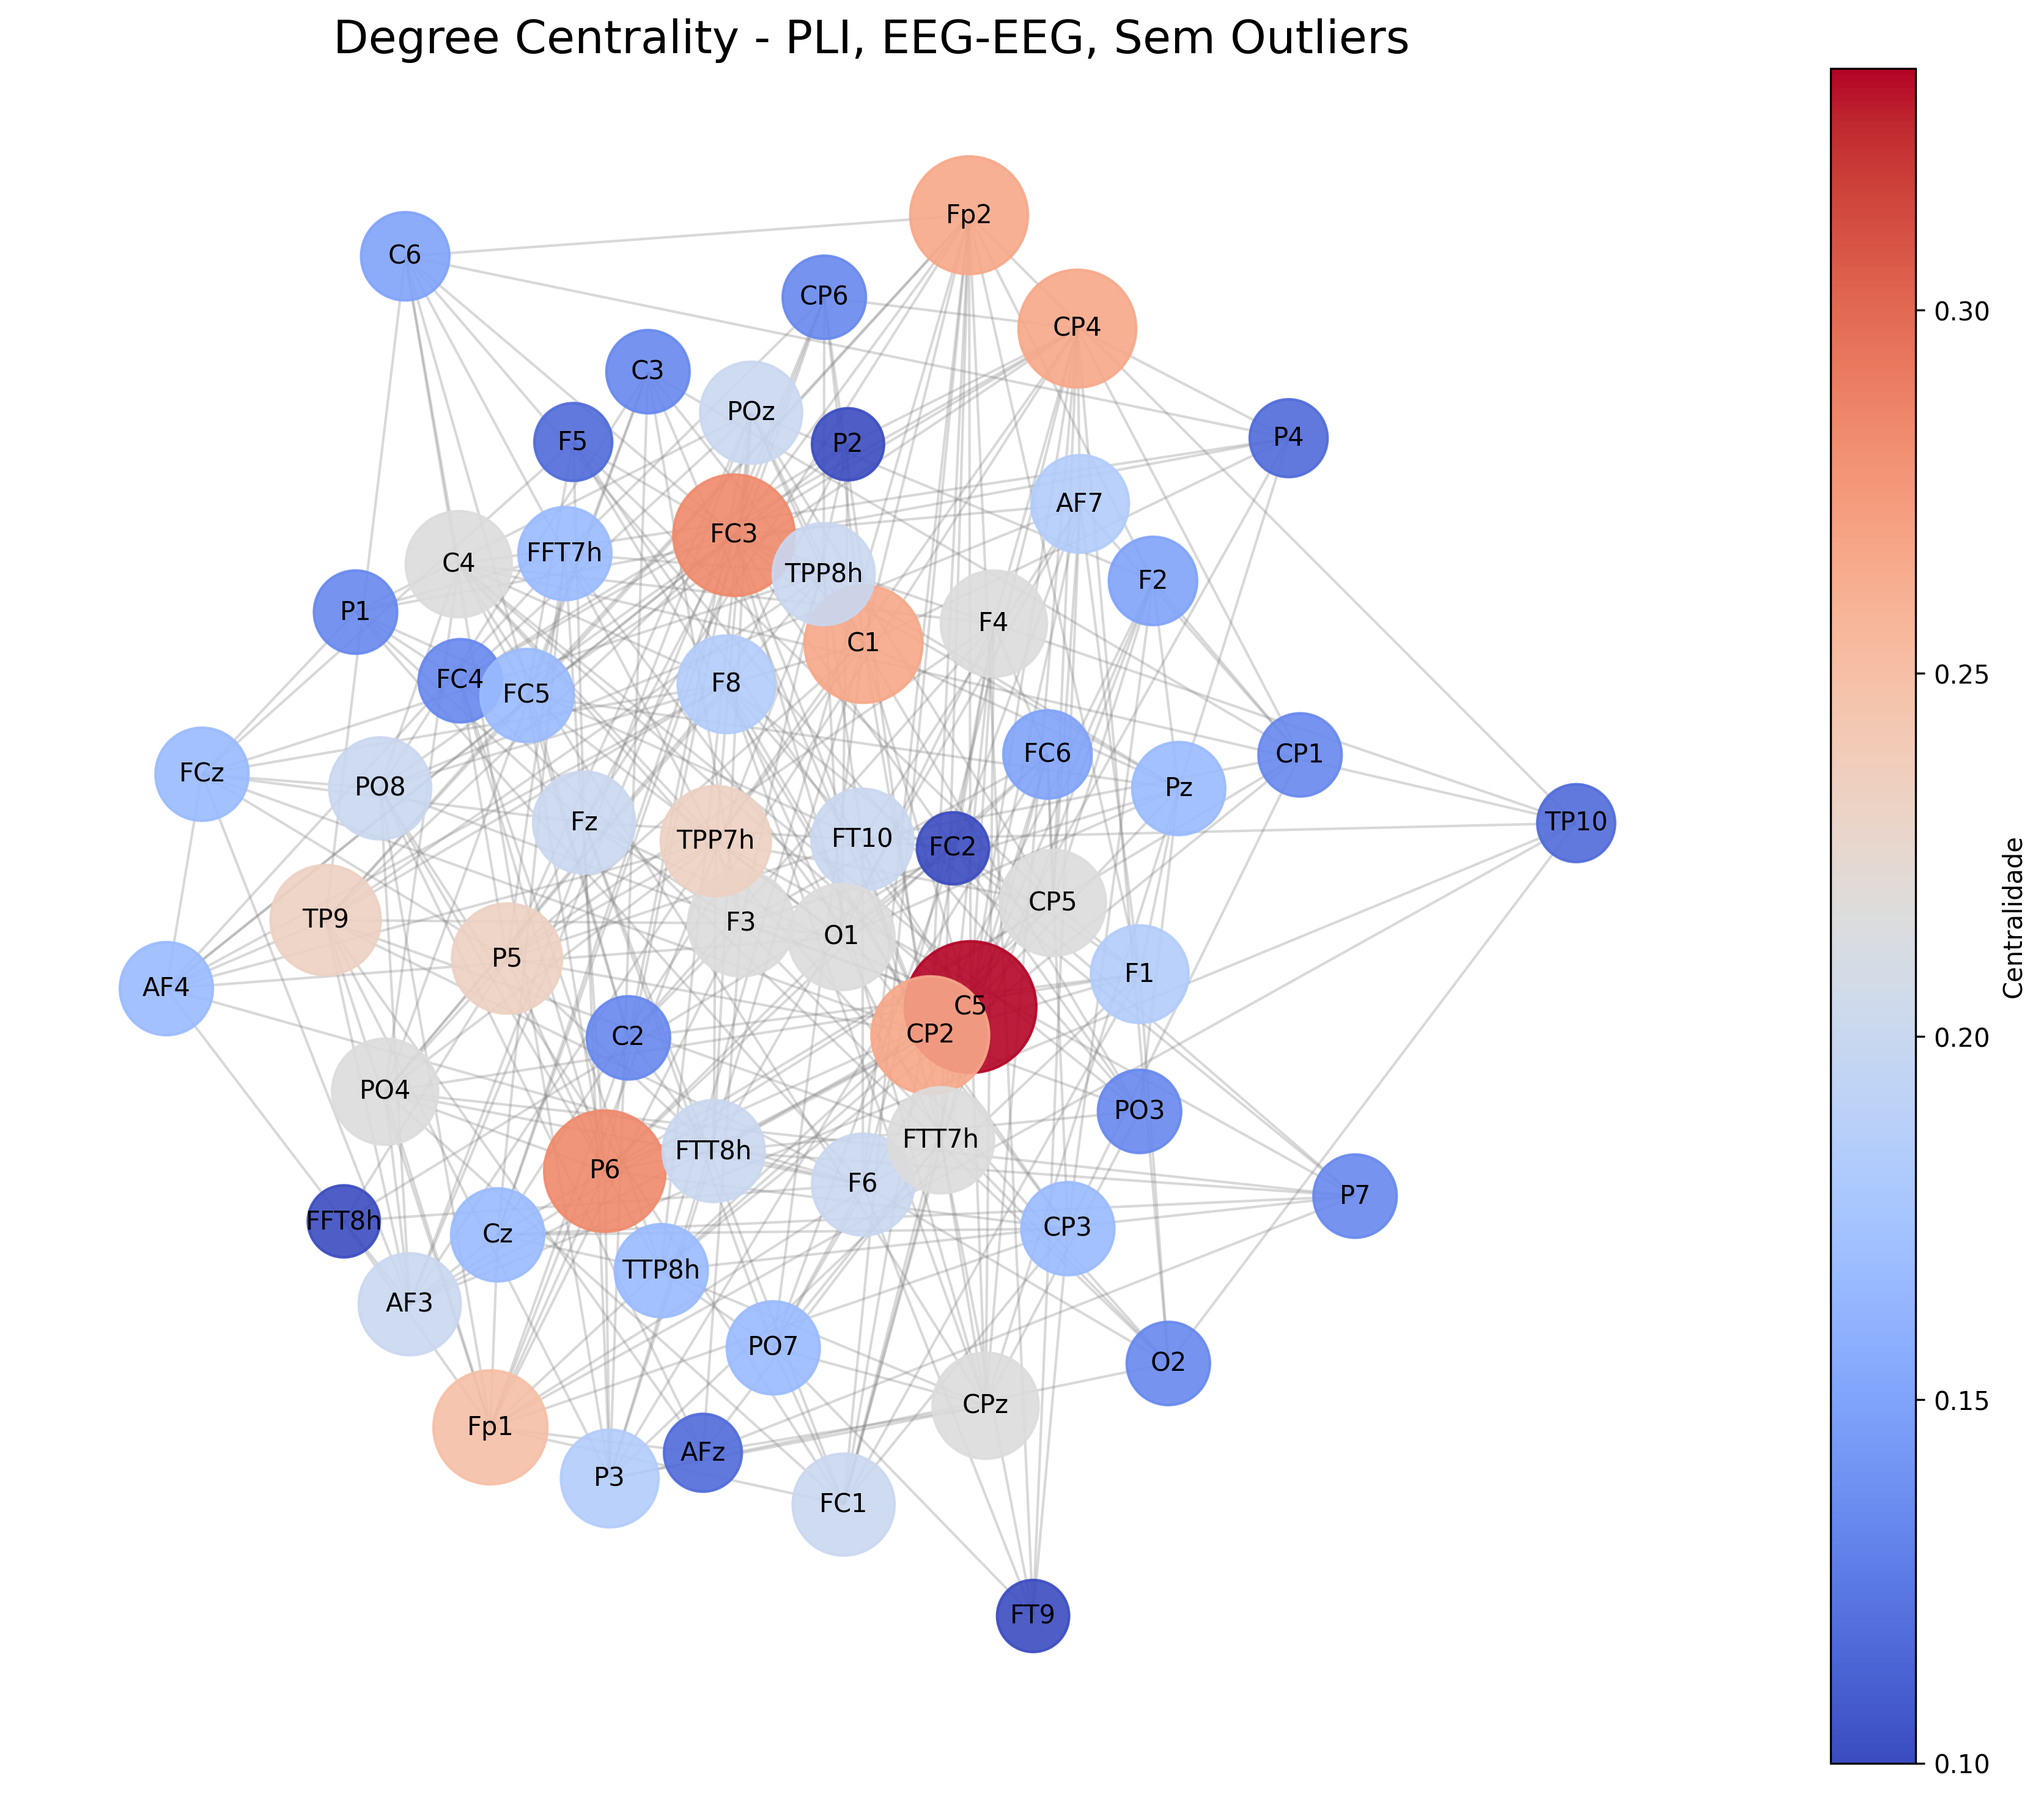
\includegraphics[width=0.45\textwidth]{figs/7_bootstrap_results_analysis/3_centrality_graphs/Degree_Centrality__PLI_EEGEEG_Sem_Outliers.png}
        \label{fig:dc_pli_eegeeg_sem}
    }
    \caption{Degree Centrality no cenário PLI (EEG-EEG). Alguns canais (por ex., Fp2, CP2) apresentam alto grau de conexões diretas.}
    \label{fig:dc_pli_eegeeg}
\end{figure}

A Figura~\ref{fig:dc_pli_eegeeg} revela que, em PLI (EEG-EEG), determinados canais (Fp2, CP2, etc.) se destacam por estabelecerem mais conexões diretas de \emph{phase lag} com outros canais. Isso sugere que tais canais podem atuar como “hubs de comunicação” \cite{newman2010networks}. No cenário sem outliers, a estrutura global é mantida, indicando a robustez do padrão de conectividade.

\subsection{Eigenvector Centrality}
A \emph{eigenvector centrality} avalia a importância de um nó considerando não apenas quantas conexões ele possui, mas também o quão importantes são os nós a que ele está conectado \cite{bonacich1972factoring}.

\subsubsection{CF-PLM (EEG-ECG)}
\begin{figure}[htb]
    \centering
    \subfloat[Com Outliers]{
        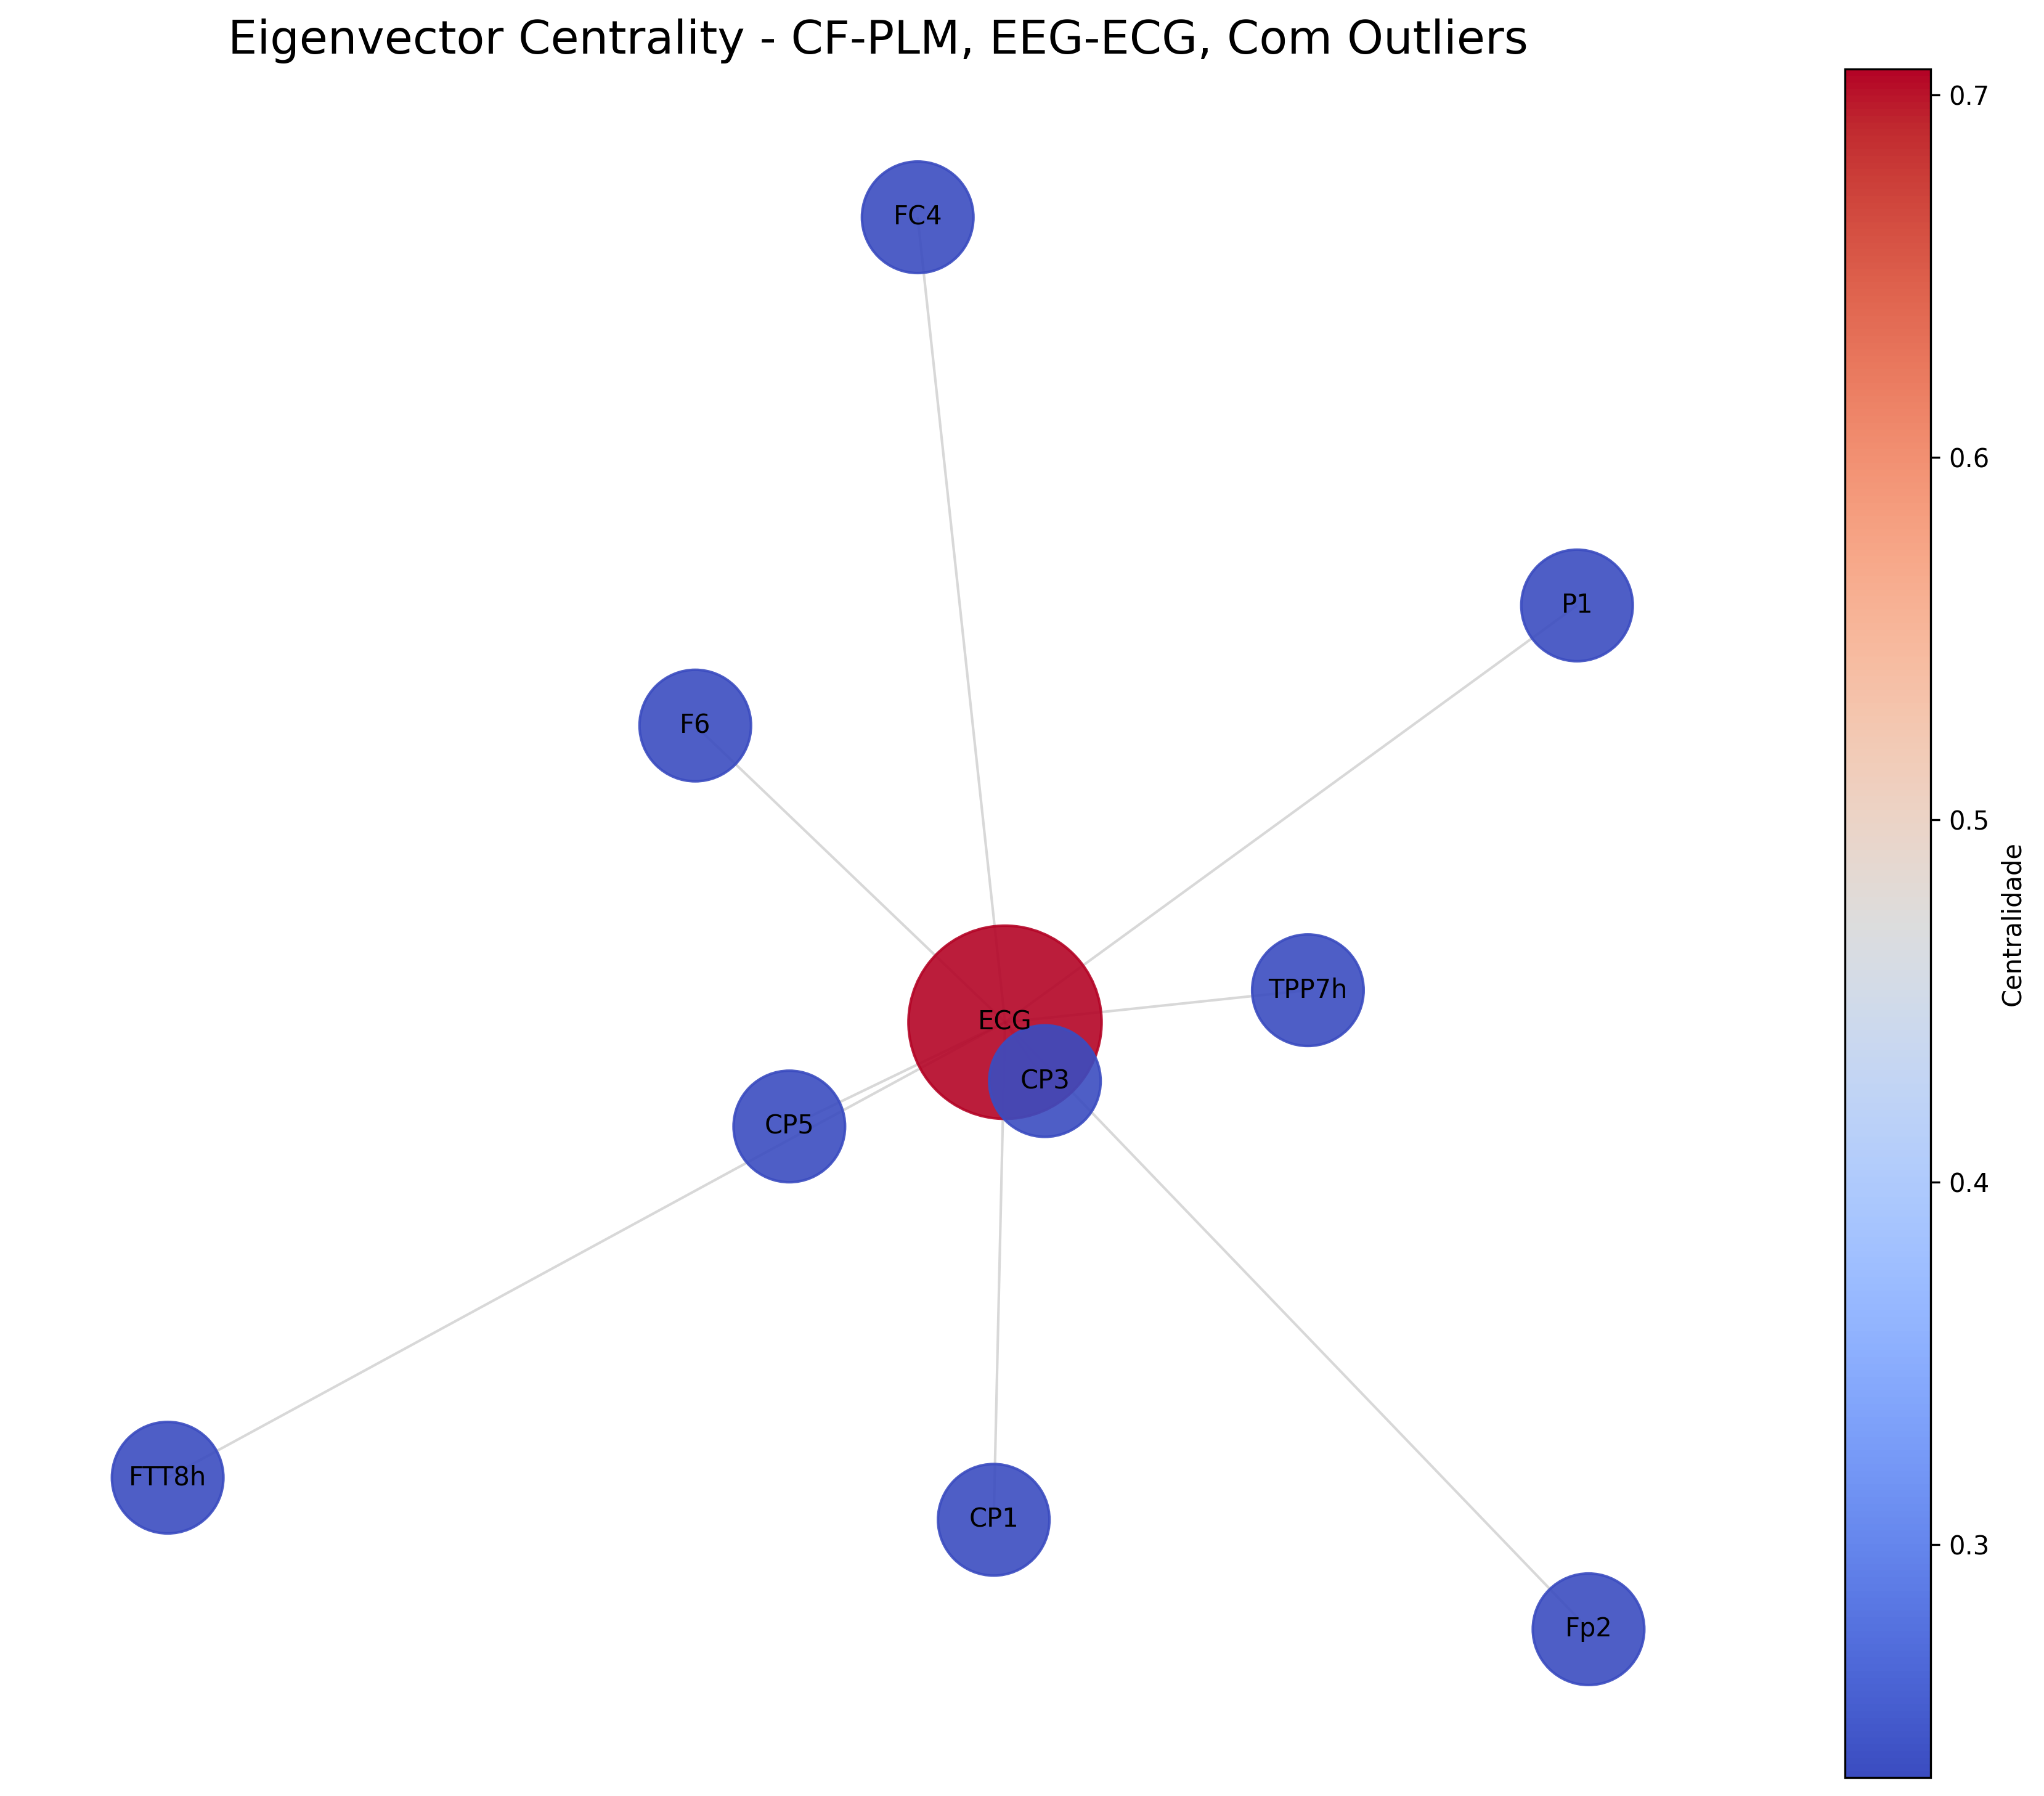
\includegraphics[width=0.45\textwidth]{figs/7_bootstrap_results_analysis/3_centrality_graphs/Eigenvector_Centrality__CFPLM_EEGECG_Com_Outliers.png}
        \label{fig:ec_cfplm_eegecg_com}
    }
    \quad
    \subfloat[Sem Outliers]{
        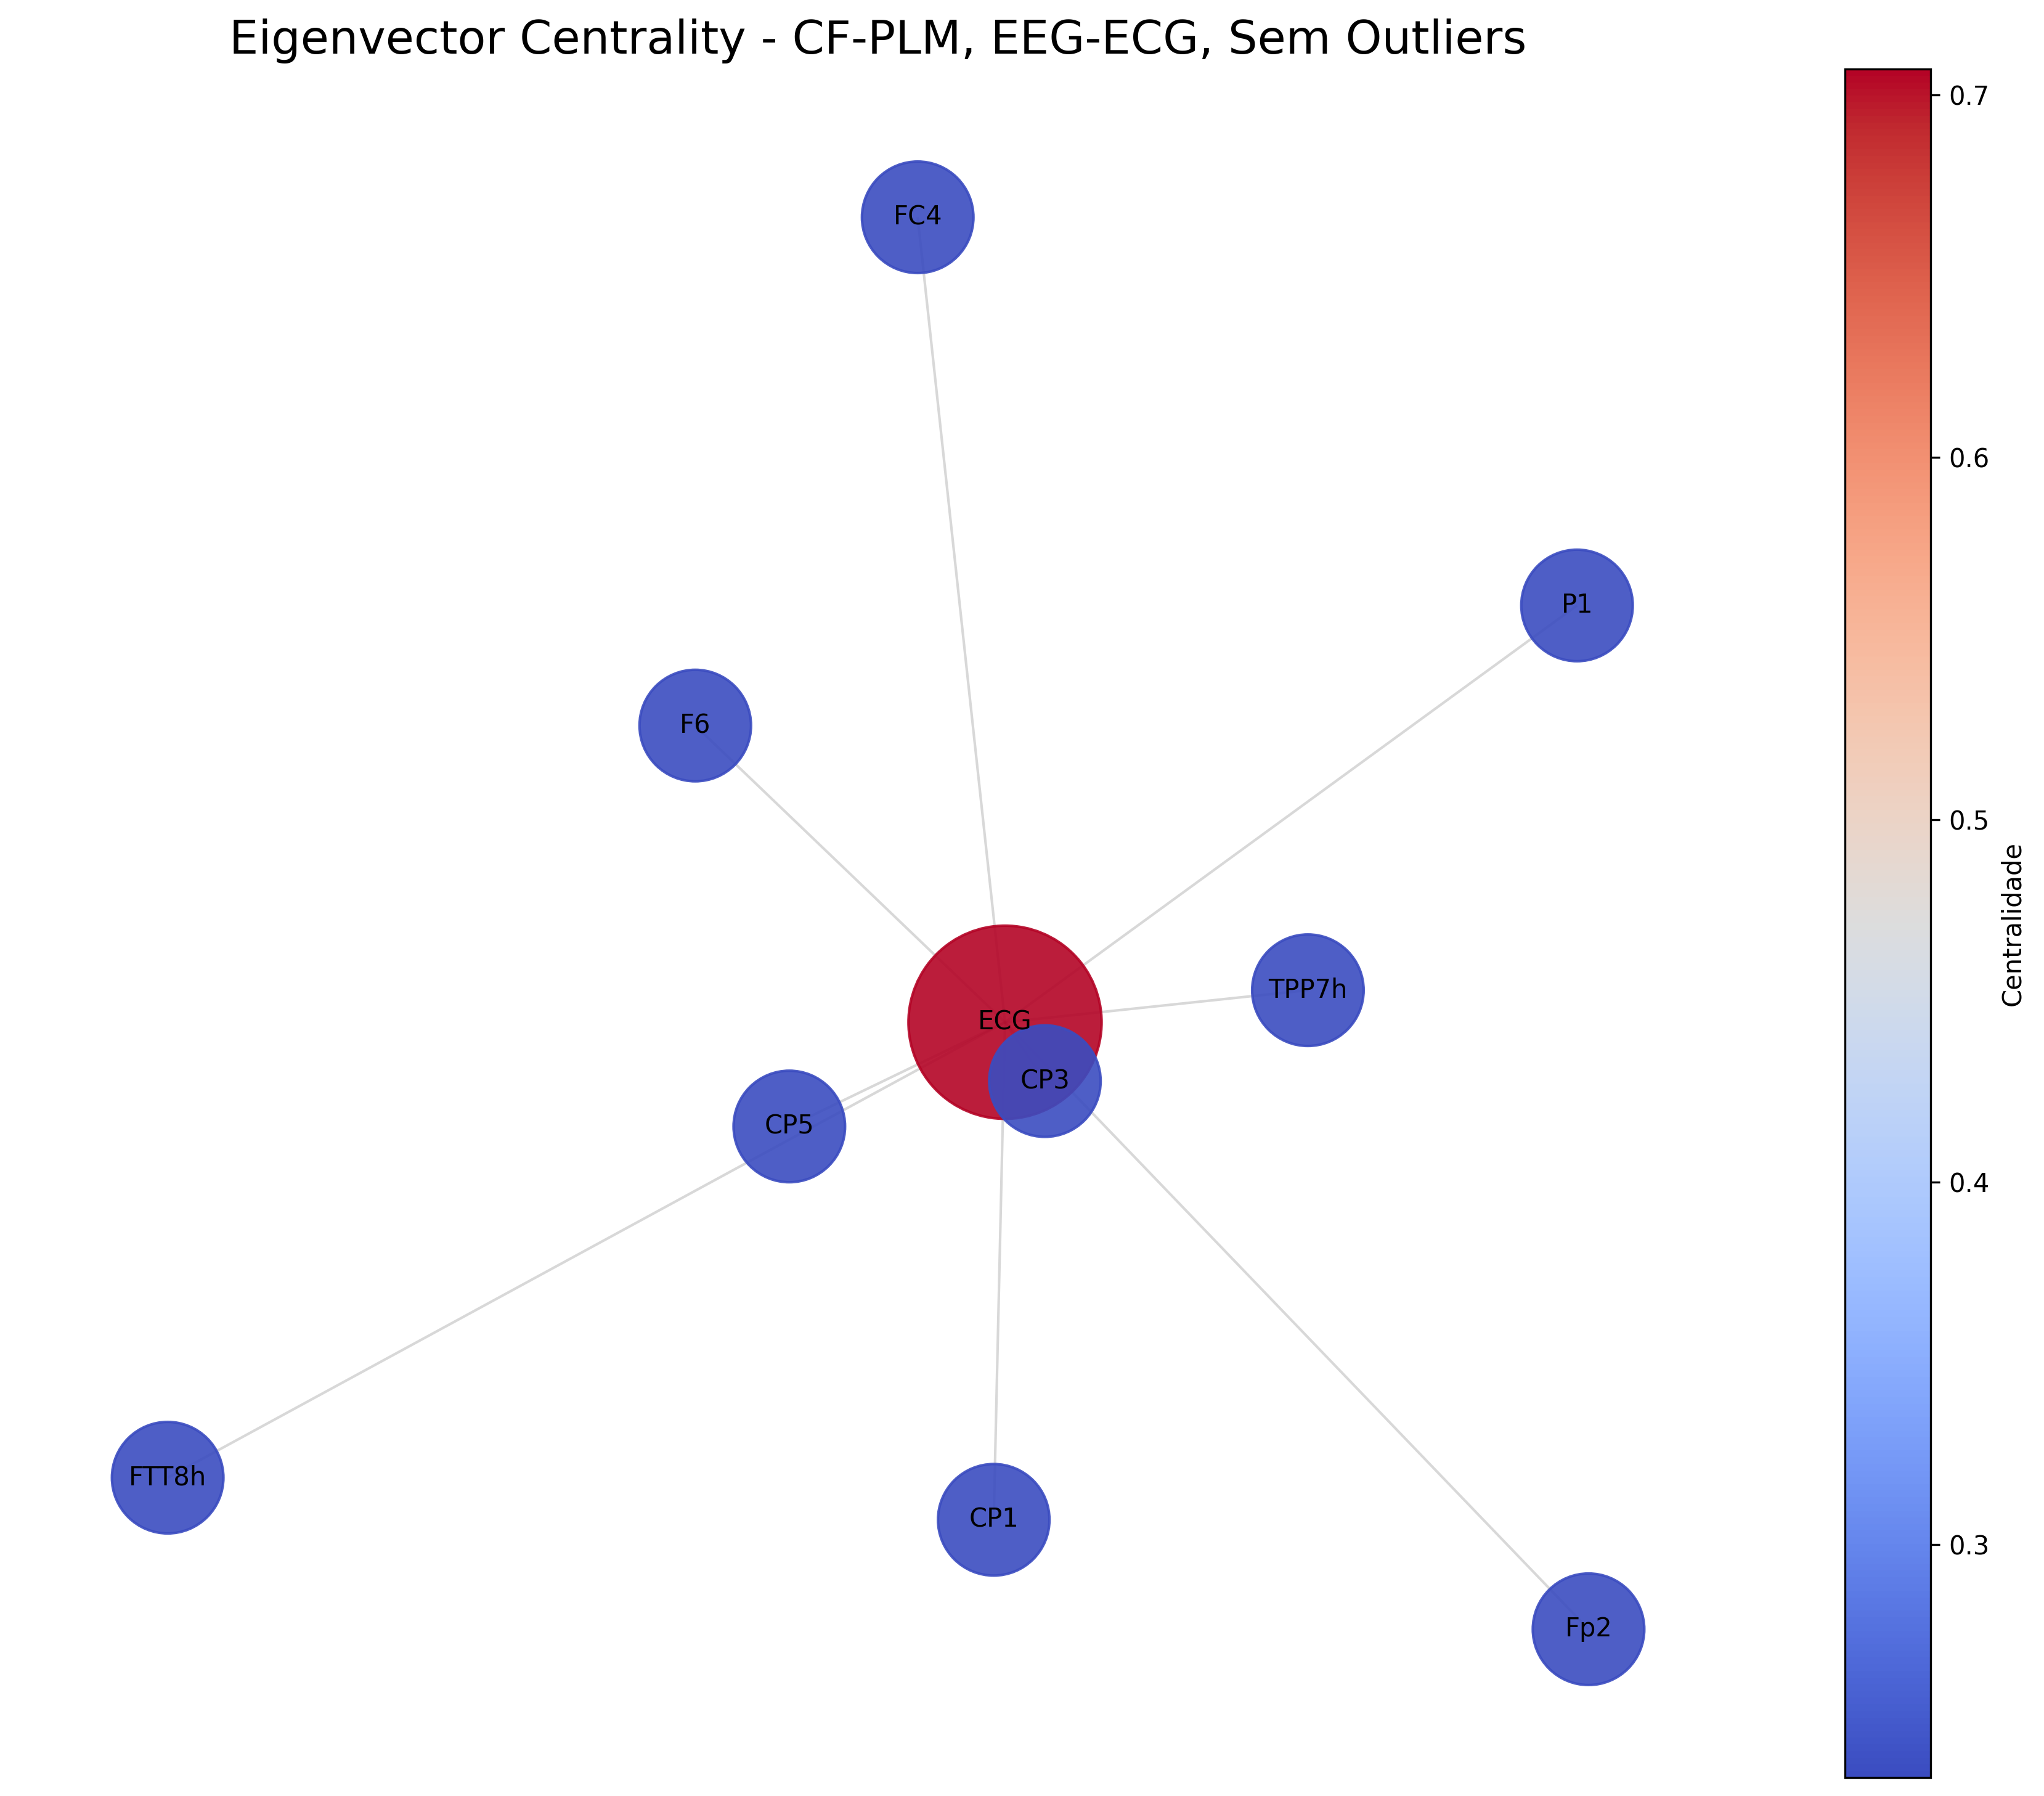
\includegraphics[width=0.45\textwidth]{figs/7_bootstrap_results_analysis/3_centrality_graphs/Eigenvector_Centrality__CFPLM_EEGECG_Sem_Outliers.png}
        \label{fig:ec_cfplm_eegecg_sem}
    }
    \caption{Eigenvector Centrality no cenário CF-PLM (EEG-ECG). O canal \emph{ECG} retém a maior centralidade em ambos os cenários.}
    \label{fig:ec_cfplm_eegecg}
\end{figure}

Conforme a Figura~\ref{fig:ec_cfplm_eegecg}, o \emph{ECG} domina a \emph{eigenvector centrality}, pois conecta-se a canais (p.\,ex.\ F6, CP5, etc.) que também são relativamente relevantes na rede. A remoção de outliers não altera esse fato, confirmando a preponderância do canal cardíaco no acoplamento \emph{cross-frequency} \cite{bullmore2009complex}.

\subsubsection{PLI (EEG-EEG)}
\begin{figure}[htb]
    \centering
    \subfloat[Com Outliers]{
        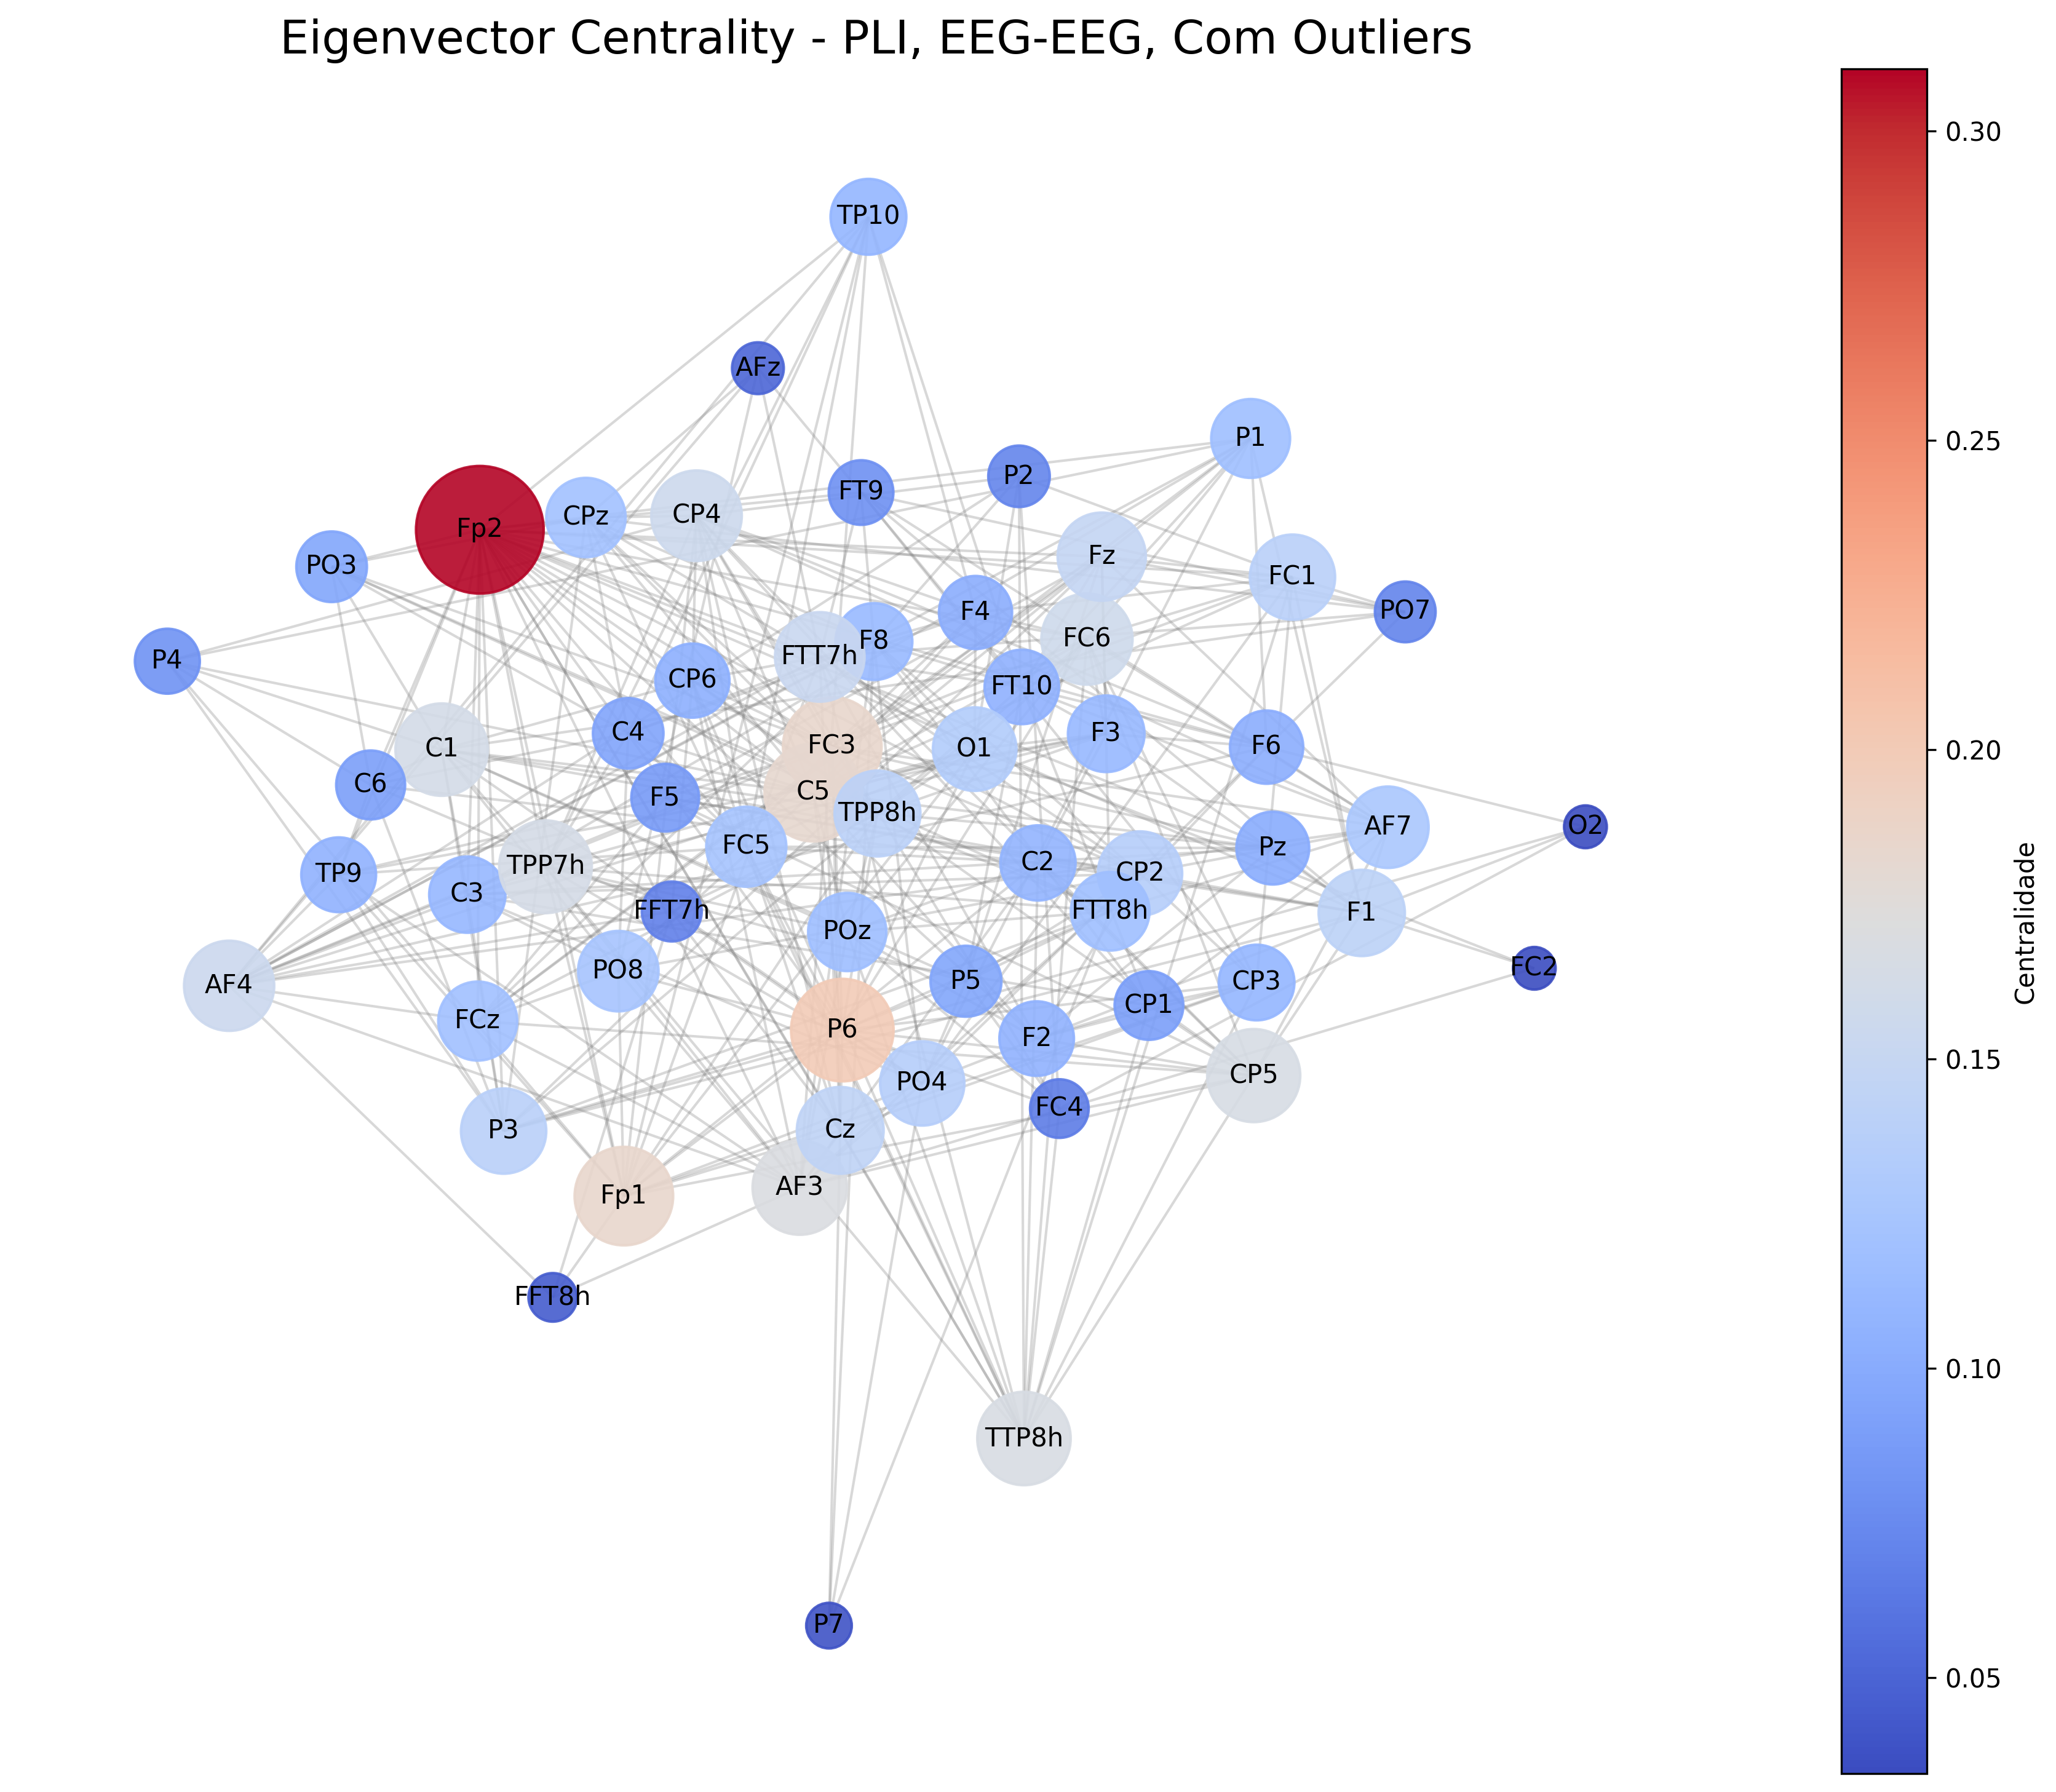
\includegraphics[width=0.45\textwidth]{figs/7_bootstrap_results_analysis/3_centrality_graphs/Eigenvector_Centrality__PLI_EEGEEG_Com_Outliers.png}
        \label{fig:ec_pli_eegeeg_com}
    }
    \quad
    \subfloat[Sem Outliers]{
        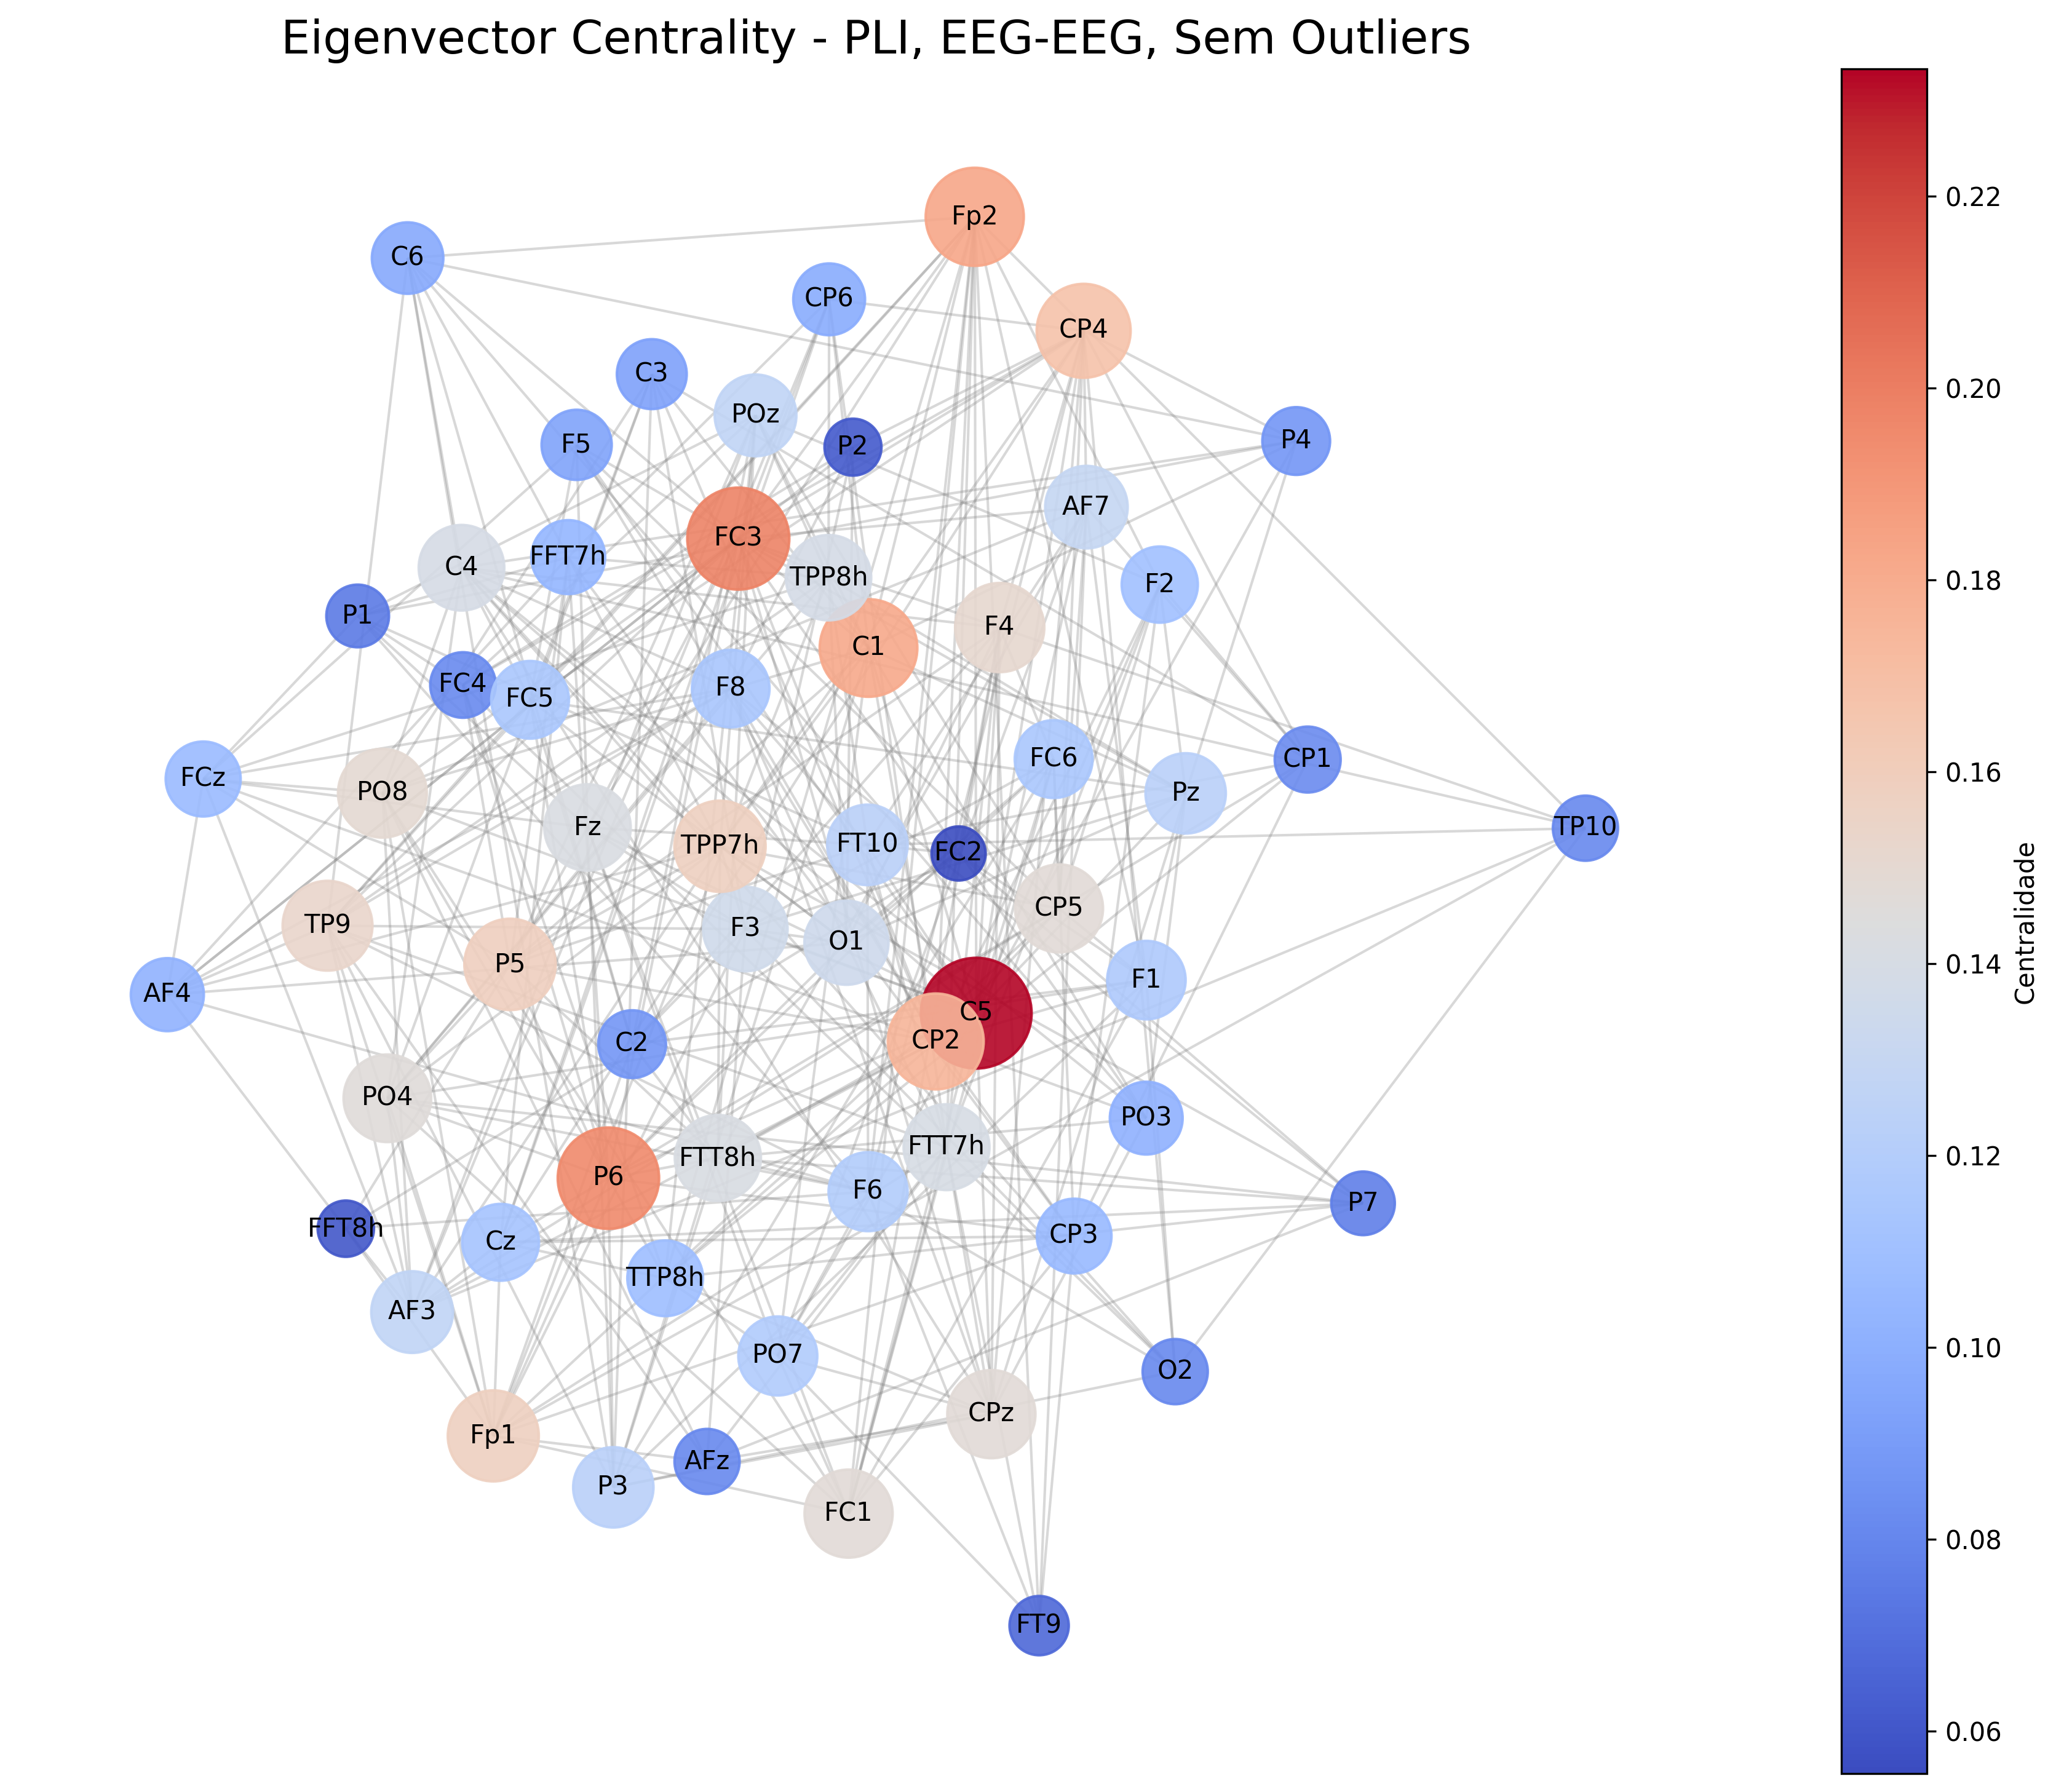
\includegraphics[width=0.45\textwidth]{figs/7_bootstrap_results_analysis/3_centrality_graphs/Eigenvector_Centrality__PLI_EEGEEG_Sem_Outliers.png}
        \label{fig:ec_pli_eegeeg_sem}
    }
    \caption{Eigenvector Centrality no cenário PLI (EEG-EEG). Alguns canais apresentam alta relevância, pois se conectam a nós também importantes.}
    \label{fig:ec_pli_eegeeg}
\end{figure}

Na Figura~\ref{fig:ec_pli_eegeeg}, canais como Fp2, CP2 ou P6 (dependendo da banda) podem surgir em destaque, pois não apenas possuem diversas conexões diretas (alto grau), mas também se ligam a outros nós centrais, amplificando sua influência \cite{bonacich1972factoring}. O cenário sem outliers não altera a hierarquia principal, reforçando a robustez da rede.

\subsection{Discussão e Comparação das Métricas de Centralidade}
\label{subsec:discuss_centrality_metrics}

\paragraph{Betweenness vs. Degree vs. Eigenvector} Cada métrica de centralidade oferece uma perspectiva diferente \cite{rubinov2010complex}:
\begin{itemize}
    \item \textbf{Betweenness Centrality}: mede o quão frequentemente um nó se encontra em caminhos mais curtos, identificando nós “ponte” críticos no fluxo de informações.  
    \item \textbf{Degree Centrality}: indica quantas conexões diretas cada nó possui, revelando os “hubs” de maior popularidade.  
    \item \textbf{Eigenvector Centrality}: pondera a importância de um nó considerando o quão importantes são os nós aos quais ele se conecta, destacando nós que influenciam ou são influenciados por outros hubs.  
\end{itemize}

\paragraph{Relações Observadas}
\begin{itemize}
    \item \textbf{EEG-ECG (CF-PLM)}: O canal \emph{ECG} domina em todas as métricas (betweenness, degree, eigenvector), pois todo acoplamento \emph{cross-frequency} passa por ele, tornando-o invariavelmente o nó central. A remoção de outliers não modifica essa hierarquia.
    \item \textbf{EEG-EEG (PLI)}: Em cada métrica de centralidade, alguns canais frontais (ex.: Fp2) ou parietais (ex.: CP2) destacam-se como hubs, seja por número de conexões (degree), seja por servirem de ponte (betweenness) ou por se conectarem a nós igualmente relevantes (eigenvector). Isso sugere que tais canais podem exercer influência significativa na sincronização de fase iso-frequencial, podendo ser alvos interessantes para investigações sobre neuromodulação \cite{bullmore2009complex, rubinov2010complex}.
\end{itemize}

\paragraph{Impacto da Remoção de Outliers}  
Em todos os cenários, a remoção de outliers teve impacto mínimo sobre a estrutura global e sobre os principais hubs. Isso indica que as conexões mais fortes e os canais mais centrais não dependem de valores extremos, reforçando a robustez das redes obtidas e das métricas de centralidade utilizadas \cite{newman2010networks}.

\paragraph{Implicações para a Dissertação}  
A análise de centralidade confirma os achados prévios de sincronização:  
\begin{itemize}
    \item No acoplamento \emph{cross-frequency} (EEG-ECG), o canal \emph{ECG} é naturalmente o nó mais importante, conectando-se a canais cerebrais que podem exibir leve variação em sua centralidade.  
    \item Na sincronização iso-frequencial (EEG-EEG), determinados canais surgem como hubs (ex.: Fp2, CP2, etc.), possivelmente refletindo o papel de regiões frontais e parietais na coordenação neural.  
\end{itemize}
Esses resultados fornecem uma base sólida para discussões sobre a influência da estimulação \emph{cathodic} e \emph{sham} em redes neurais e na interação cérebro-coração, indicando possíveis regiões de interesse para estudos futuros e correlações com desempenho comportamental \cite{bullmore2009complex, rubinov2010complex}.

\bibliographystyle{abntex2-alf}
\bibliography{bibliography}
